%\documentclass[journal=jpr,manuscript=article]{achemso}
\documentclass{article}
\usepackage[margin=0.5in]{geometry}
\usepackage{graphicx}
\usepackage{mathtools,amssymb}
\usepackage{color}
\usepackage[english]{babel}
\usepackage{authblk}
\usepackage{url}
%\usepackage{soul}
\usepackage[ruled,vlined,linesnumbered]{algorithm2e}
\usepackage{algorithmic}


%\graphicspath{{figs/}}  Store figures at the level of the main doc
\newcommand{\argmax}{\text{argmax}}
\newcommand{\todo}[2]{{\color{red} {\bf TODO-#1}: #2}}
\newcommand{\comment}[2]{{\color{blue} {\bf Comment-#1}: #2}}
\newcommand{\correction}[2]{{\color{red} \st{#1} }{\color{red} #2}}
%\newcommand{\correction}[2]{#2}  % Use this to make a document with hiding track changes.

%\usepackage[backend=biber,style=nature,articletitle=false]{biblatex}
%\usepackage[backend=biber,style=nature]{biblatex}
%\addbibresource{bibliography.bib}

%\usepackage[backend=biber]{biblatex}
%\usepackage{natbib}
%\addbibresource{bibliography.bib}
\newcommand{\pe}[0]{\mathrel{{+}{=}}}

\usepackage{setspace}
\doublespacing
%\newcommand*{\DOUBLEBLINDREVIEW}{} %Uncomment to hide author information for double-blind peer review


\author{Andrey Borevsky}
\author{Attila Kertesz-Farkas$\ast$}
\affil{Laboratory on AI for Computational Biology, Faculty of Computer Science, HSE University,  11 Pokrovsky Bvld., Moscow 109028, Russian Federation}
%\email{akerteszfarkas@hse.ru}
%\phone{+7 (499) 152-07-41}

\title{Utilizing exact p-values for improved classification and accurate false discovery rate control}

\begin{document}

\maketitle

\begin{abstract}
Exact p-value (XPV)-based methods for dot product-like score functions ...


\end{abstract}
\textbf{Key words:} Exact p-values, empirical p-values, False discover rate control, classification, score calibration

\section{Introduction}

Classification is a renown machine learning task, being enriched throughout last decades with various metrics. Each of them expects a growth only with the simultaneous enhancement of the model’s classification power, revealing a certain level of effectiveness. Meanwhile, a broad family of evaluation approaches has been introduced to present a comprehensive analysis.

It is vital to distinct two basic types of errors, which could be made by a classification method. If implying existence of two classes only, then the model might either propose a negative sample to be positive (false negative, FN) or vice versa (false positive, FP). Usually, the type of mistake is indifferent to the inference. However, some situations require diametrically opposite evaluation policy. For instance, we could dive into the biomedical sphere, such as brain cancer. A neural network processes snapshots of living-patient’s brain cells, searching for those infected. Hence, separating two kinds of error is of paramount importance. Incorrectly recognizing healthy cells as rogue ones (FP) is much more hazardous since the surgeon will remove a wrong part of a brain - action, which can not be undone. So, there is a pool of applications that demand extremely strict control of the extent to which the algorithm makes FP mistakes. In such cases, False Discovery Rate (FDR) appears to be preferable.

The false discovery rate is the expected proportion of falsely classified data, whereas a false discovery is a data instance that is misclassified. 

Some FDR control methods rely on knock-off \todo{akf}{Check these knock off methods} or decoy samples. Perhaps, other types of FDR control methods rely on accurate p-values associated to each prediction.

We intend to elaborate a specific approach to produce uniformly distributed p-values for test data that would establish a consequent FDR control. Thus, we strive to take statistical methods of bioinformatics and dive into a broader area of ML classification.

The aim of this study:
\begin{itemize}
	\item Demonstrate the accuracy of the empirical p-values,
	\item Accurate FDR error control can be achieved without class labels on the test data.
	\item it can be used to detect distribution shift in the test data. 
\end{itemize}

\section{Methods}

It is important to keep it in mind that methods reporting p-values using either analytical models (such as normal distribution) or some empirical methods are just merely estimations/approximatinos of the true but unknow p-values. If a p-value estimation method systematically produces more significant p-values, i.e. smaller numbers, than the true (but unknown) p-values, then it is called a liberal or optimistic; if it systematically produces less significant p-values, i.e. larger numbers than the true p-values, it is called a conservative estimation. Luckily, there is a way to asses the bias in p-values. It is known that, sampling from a distribution, the corresponding p-values are uniformly distributed. In order to show this, let us assume we are given a continuous, cumulative distribution function $F_X(X)$ and it is invertible, i.e. $F_X^{-1}$ exists. We want to show that, the p-values $Z = 1-F_X(X)$ are uniformly distributed, that is $F_Z(X)$ is uniformly distributed. Note that $Z\in [0,1]$. For the uniform distribution on $U\sim U_{[0,1]}$, we also have $1-U\sim U_{[0,1]}$ uniformly distributed, furthermore $P(U\le u)=u$ and $P(U>u) = 1-u$ for any $u\in[0,1]$. Thus,
\begin{equation}
	F_Z(u)=P(Z \le u) = P(1-F_X(X)\le u)= 1-P(X\le F_X^{-1}(u))=1-F_X(F_X^{-1}(u))=1-u.
\end{equation}

Therefore, one can draw a QQ plot of the p-values against the theoretical uniform distribution for visual verification.

In this paper, we propose to use the training data to produce a null distribution $N_0$ and for a given prediction score $s$ we define the p-value as $P_{N_0}(s)=\frac{|\{x\mid x>s, x \in N_0\}|}{|N_0|}$, where $|.|$ denotes the cardinality of set. Using these p-values, the false discovery rates can be controlled, for instance, with using the Benjamini-Hochberg protocol. We note that, the aim of this study is the investigation of the p-values, and we will use the BHP as a tool to demonstrate that these empirical p-values can be used to control the FDR; however, other FDR control methods could be used, for instance, for correlated p-values, etc. 

\todo{AKF}{the introduction and the methods sections are quite rudimentary. The need rearrangement.}

The FDR control could potentially be carried out by controlling the FDR on the training data at a user defined $\alpha$ level and selecting the corresponding score as a threshold $t$. A test data achieving a prediction score less than threshold $t$ could be rejected, etc. The major issue with this approach is that, it does not adapt neither to the class distribution nor to the data distribution shifts. the method we propose here adapts to when the proportion of the positive and negative classes changes, or it can visually detect data distribution shifts. 


\section{Data and methods}

We are working solely on the ubiquitously known MNIST dataset, a rich collection of handwritten digits, becoming a baseline for any classification task nowadays. It contains 60k samples for the training stage and only 10k for the test, where all classes (from 0 to 9) are evenly distributed. Also to be mentioned is the strict normalization of the digits in the image in terms of size and centering, so the algorithms receive unified examples as input.

We have accomplished all our experiments through a standard convolutional neural network. It comprises two convolutional 2d layers, both with 8 channels, kernels of size 3 and two-step strides. Single rectifier activation function is following each of them.  The output layer is represented by a simple linear unit, providing as much classes, as it was initialized by the user.   

Model is trained with Adam optimizer with a learning rate equal to 0.01 and a BCEWithLogitsLoss cost function unless otherwise specified. The motivation for introducing such a naive model was straightforward: if we find ourselves able to ameliorate a particular quality compared to the ground truth via an elementary model on the resolvable MNIST dataset, then we could extend our approach to more comprehensive real-life tasks and models.

The entire algorithm was written on the PyTorch framework and includes several key stages throughout all separate local experiments. If formalizing our goal, then we could express our dataset as $(X_i, Y_i)_{i\in\{1, ..., n\}}$, where $X_i \in \mathbb{X}$ is a feature vector and  $Y_i \in \mathbb{Y}$ is the labels. For instance, $\mathbb{X}$ can be images and $\mathbb{Y}$ - the corresponding classes. Thus, our machine learning model becomes in some sense a comprehensive function $f$, such that $\\ f(\mathbb{X}): \  \mathbb{X} \rightarrow \mathbb{Y}$.

However, besides only generating uniform p-values, we need an understanding of the algorithm’s efficiency. Thus, we introduce two types of graphs: the “QQ” plots and the “FDR control” plots. The former depicts p-values from the uniform distribution for visual verification. We plot these p-values obtained with negative training data and their rank along the x-axis for both training (simply a diagonal) and test data. The closer our test samples get to the ideal line, the better our EPV approach operates. The second type of graphs visualizes the number of trusted classifications depending on the FDR when it is controlled with true labels (baseline) and with the BH protocol using the p-values. We also add rival LTT framework, representing the FWER methodology. As we progress towards the ground truth, our ability to function without test labels will improve as well as our capacity to forecast.


\section{Experiments}

\subsection{Classical case}

\begin{figure}
    \centering
        \begin{tabular}{ccc}
 		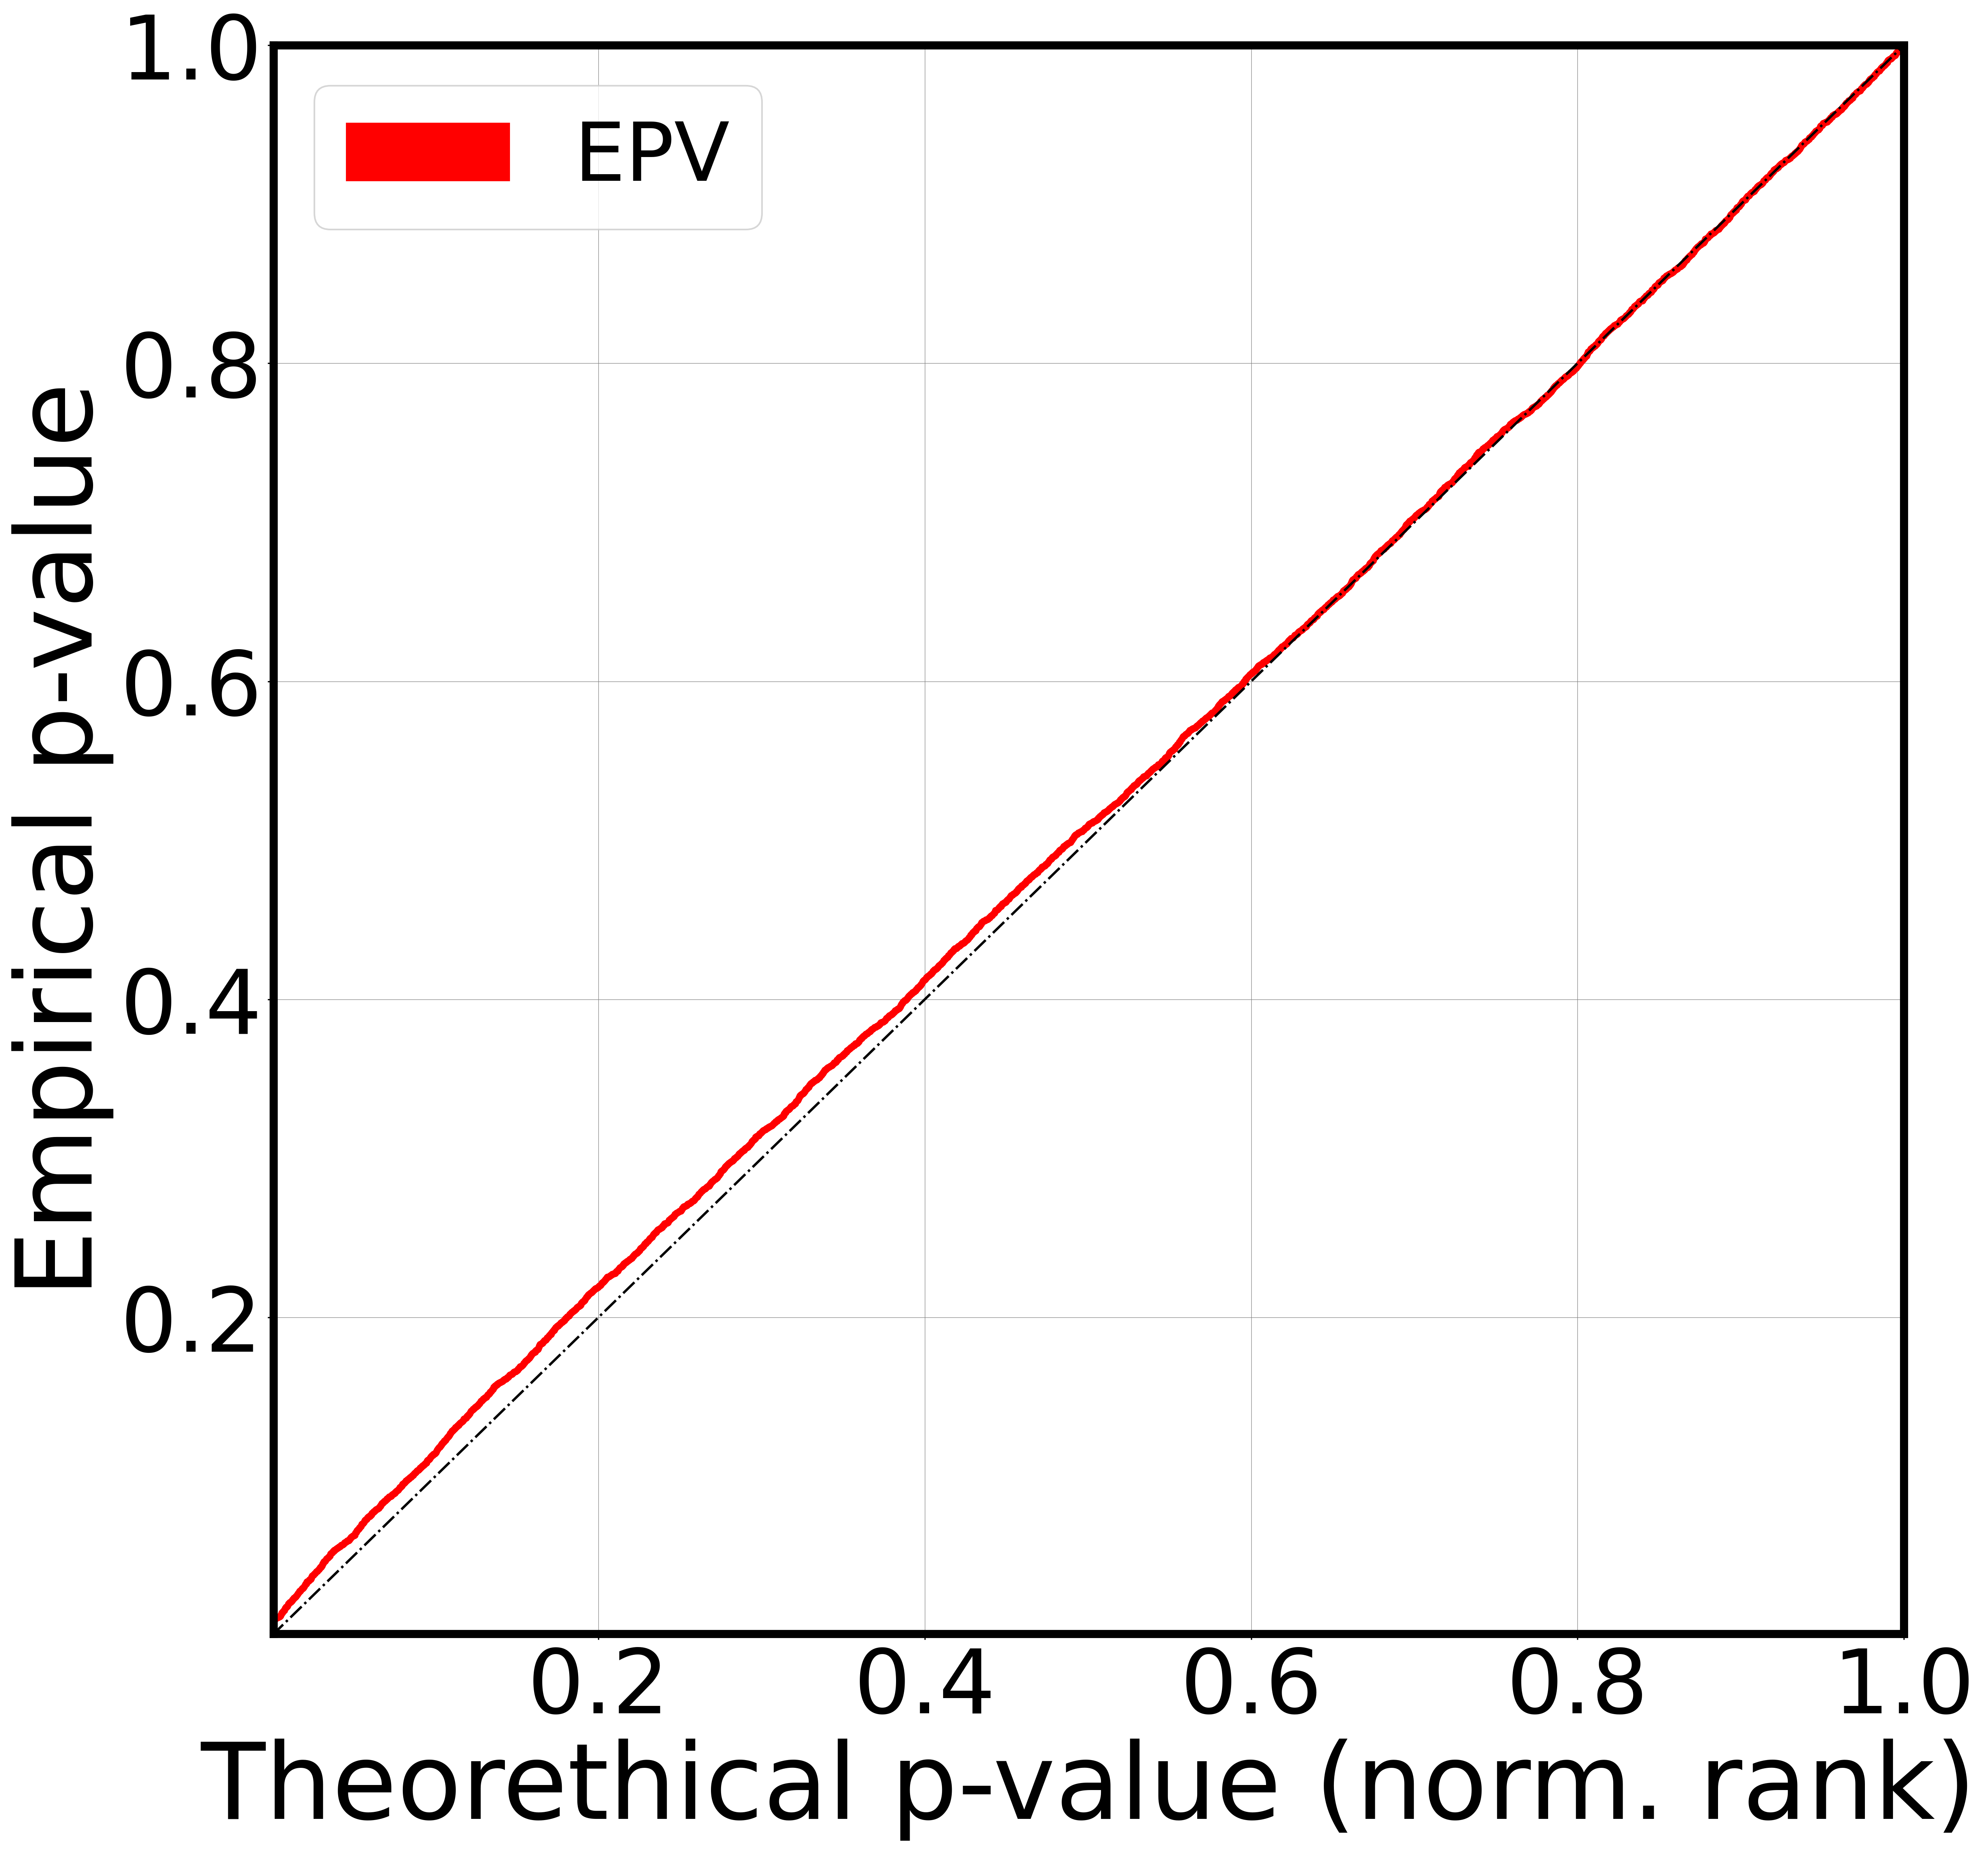
\includegraphics[width=2in]{img/cnn_QQ_classical.png} &
		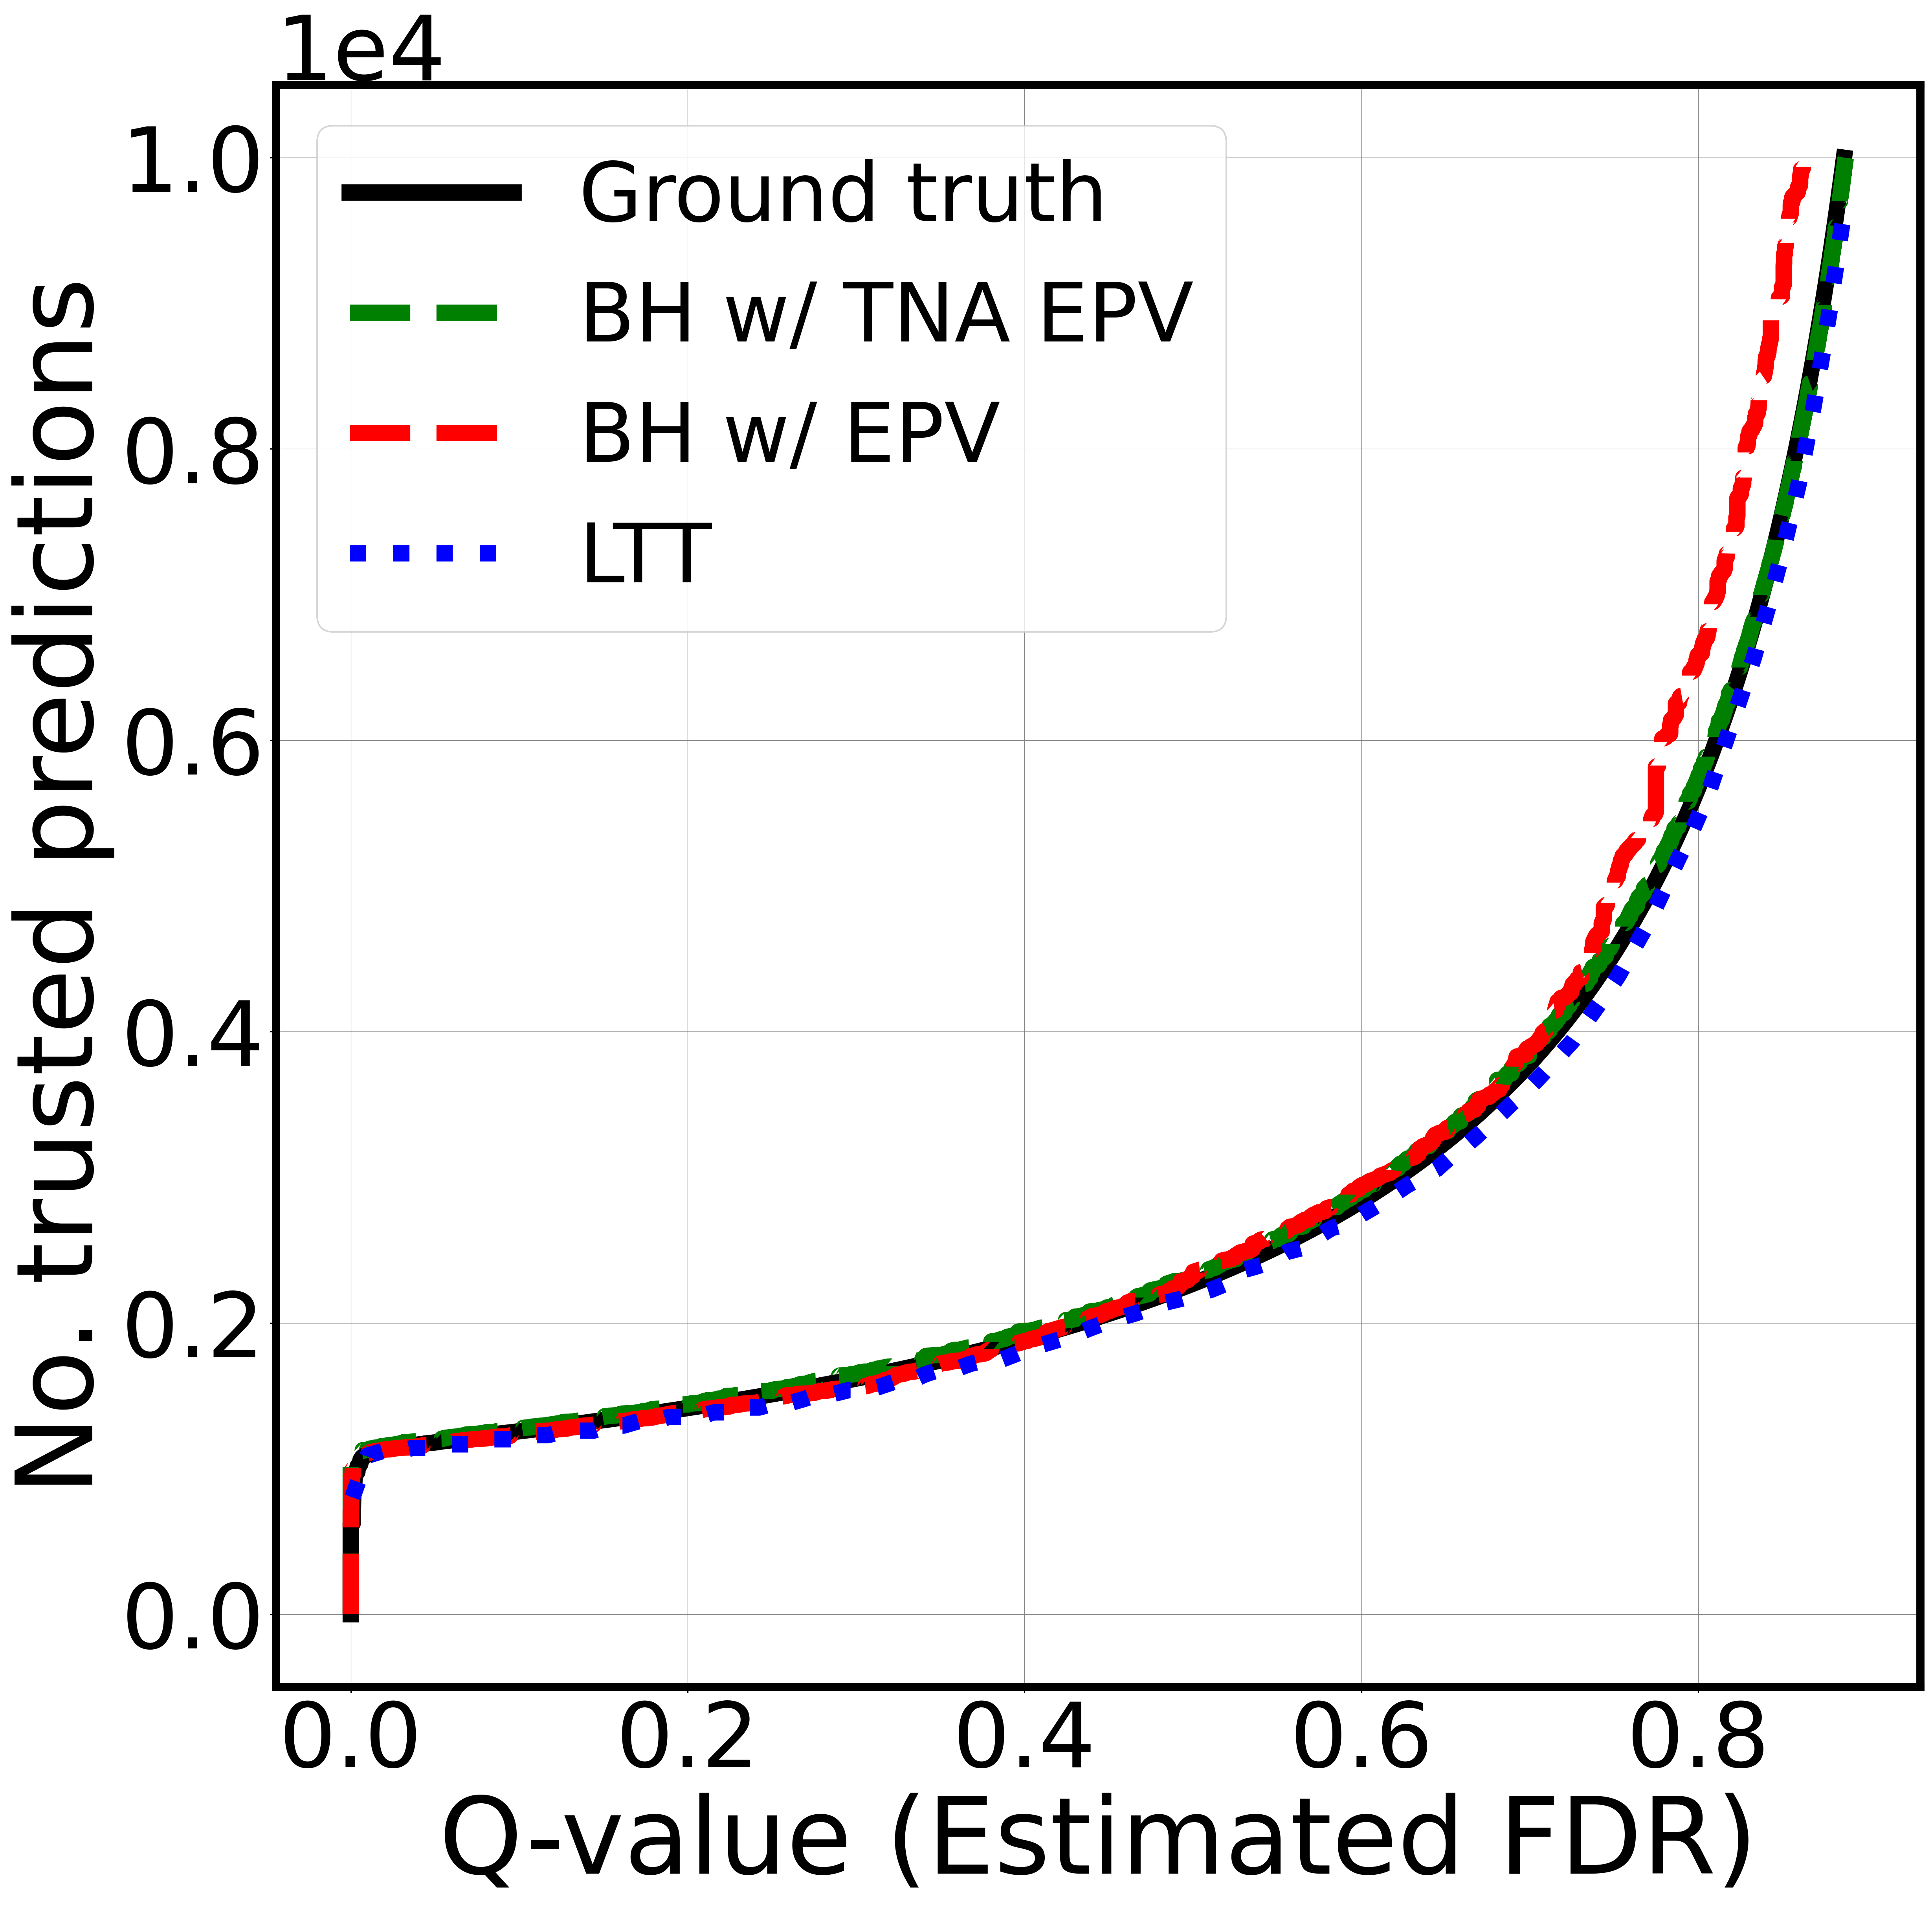
\includegraphics[width=2in]{img/cnn_classical_fdr_control.png} & 
            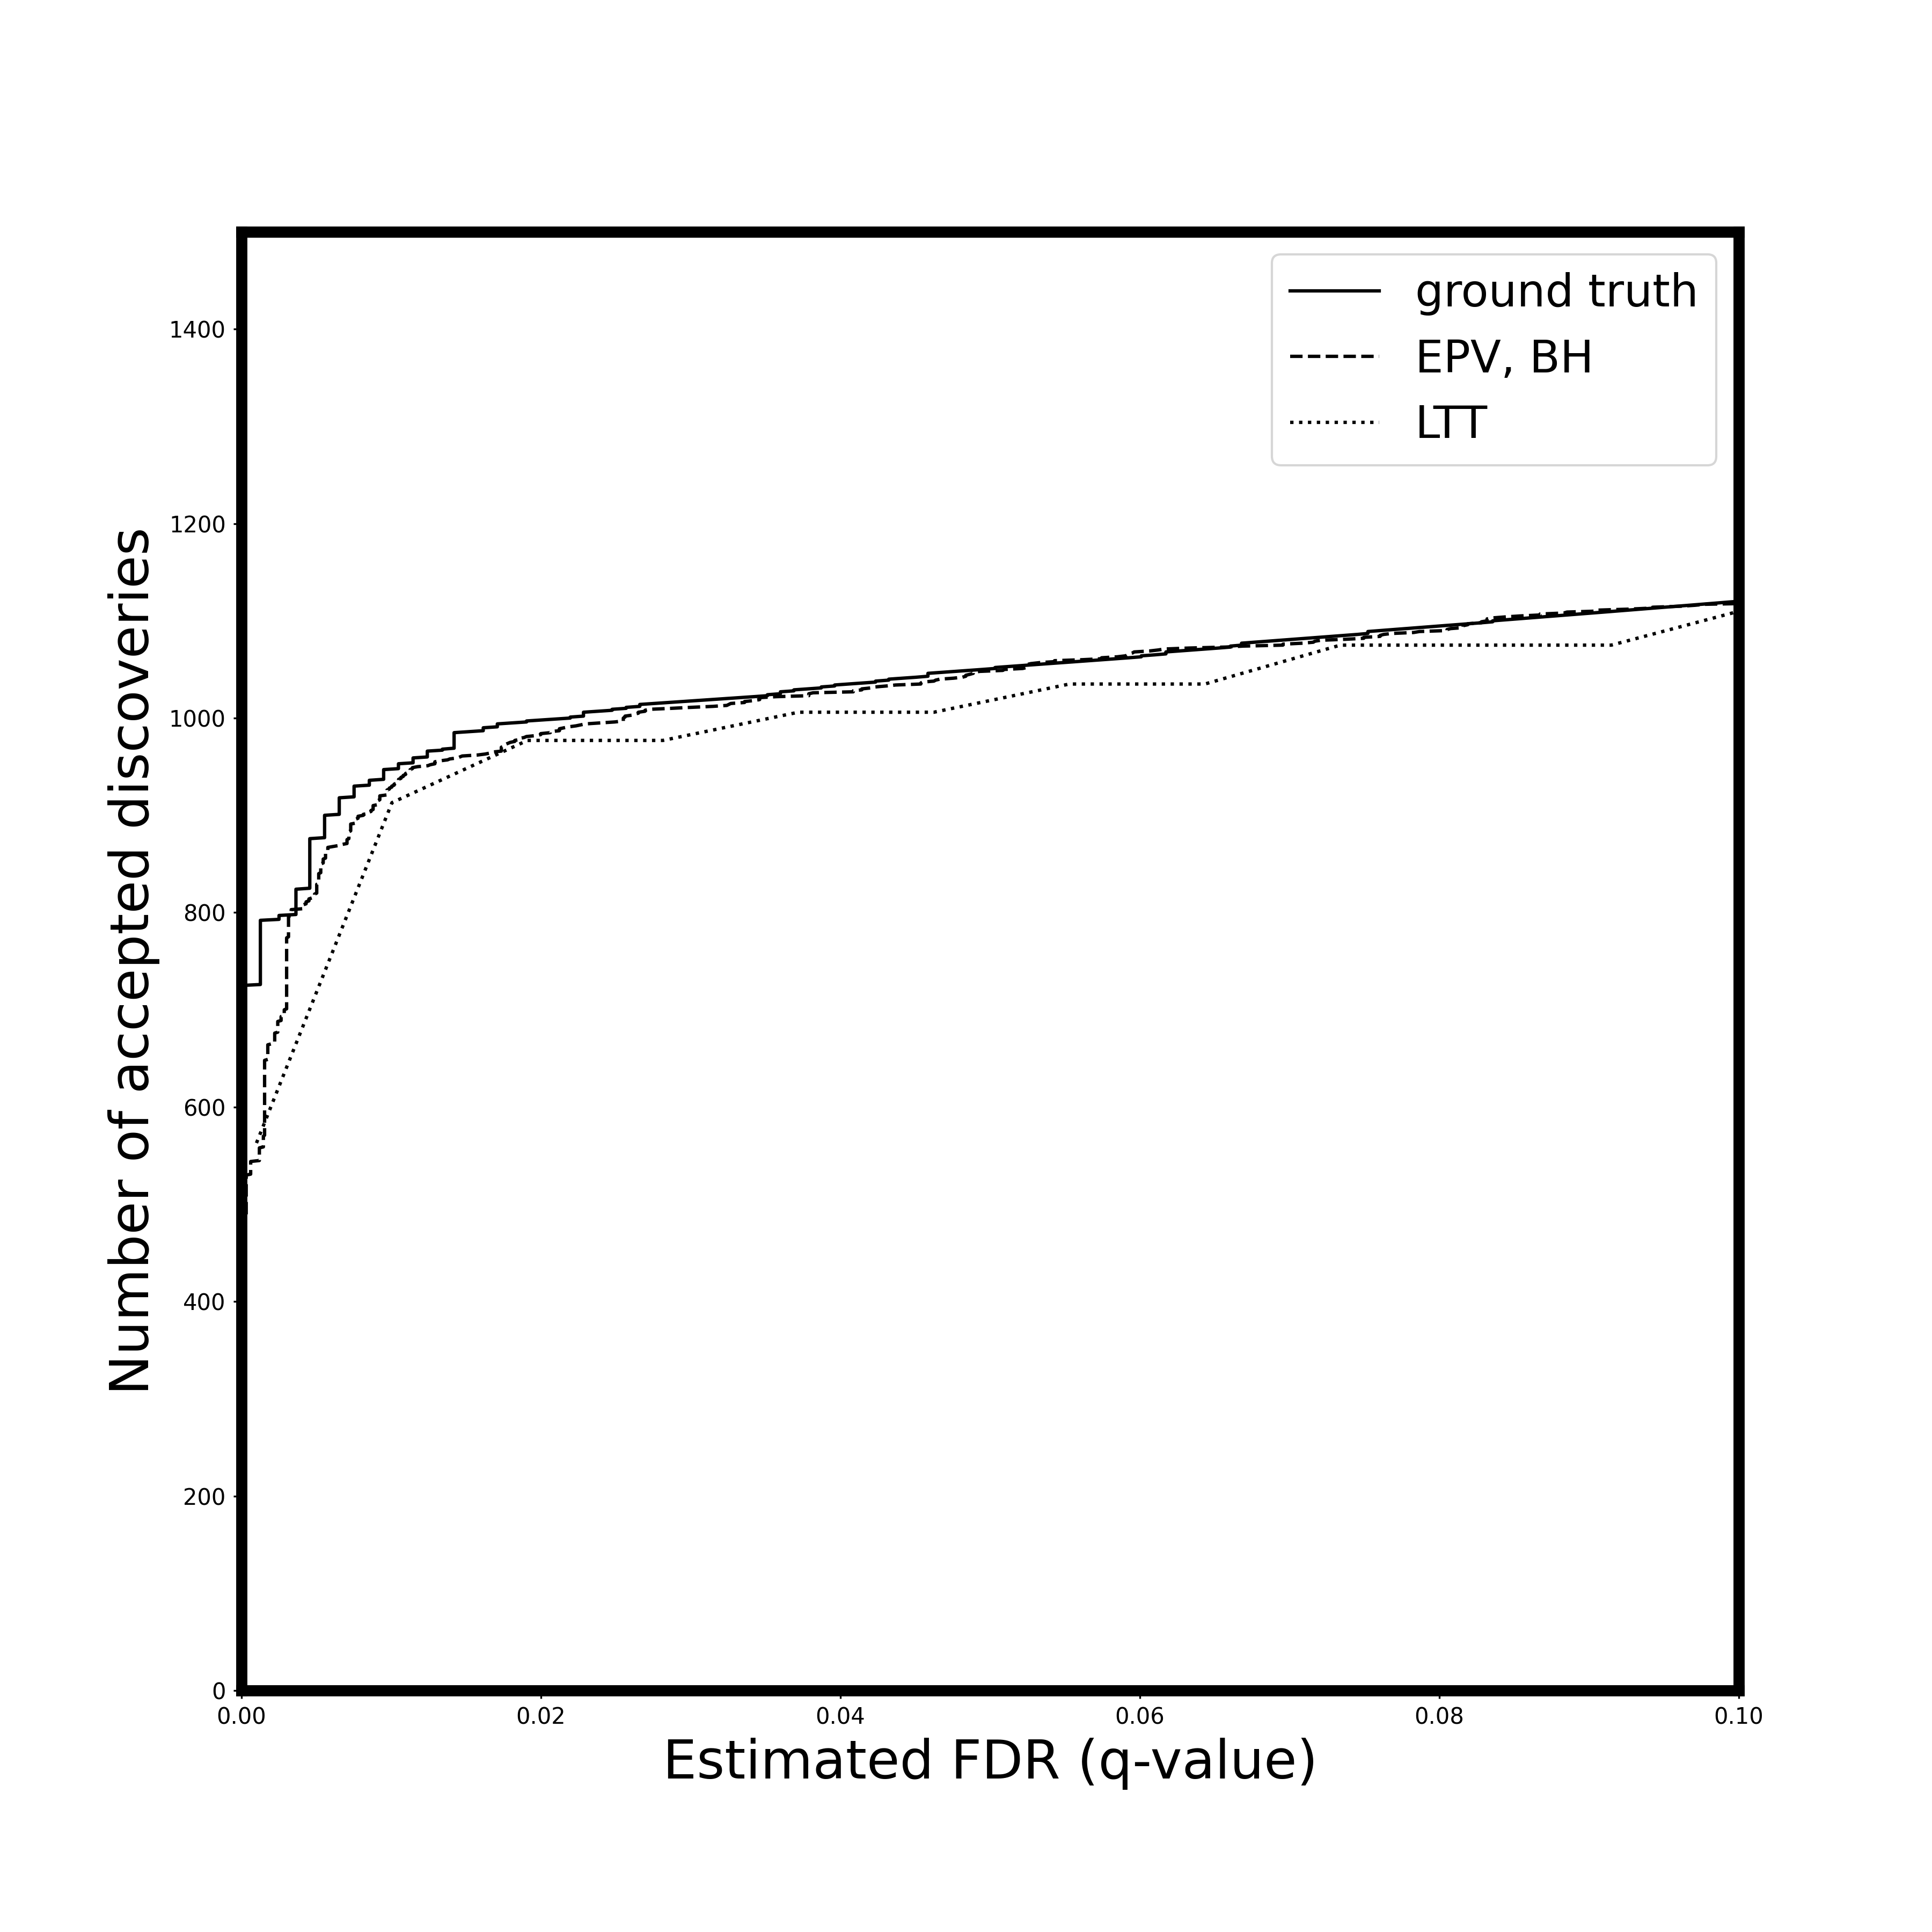
\includegraphics[width=2in]{img/cnn_classical_fdr_control_loc.png}
		\\	
		A & B & C
	\end{tabular}
	\caption{{\bf  FDR control with p-values.}
        (A) a QQ plot of the p-values obtained with using negative training data. (B) The number of trusted classifications as a function of the FDR when it is controlled with true labels (black line), with BHP (red line) and LTT (blue line) using the p-values from panel (A).
        (C) corresponds to the local range of graph (B).
        }
	\label{fig:classical}
\end{figure}

Binary classification is a basic task, where $\mathbb{Y} \in {0, 1}$. Hence, both training and test sets can be easily divided into negative and positive parts. Speaking of the MNIST dataset, we get 10\% for a positive class despite our choice for the target label, not playing any crucial role for our research. We arbitrarily chose the class "2" as a positive one, and all the samples corresponding to other classes were treated as negative data. 

The results for this most straightforward situation in context of MNIST dataset is presented on the \ref{fig:classical}. "Classical" stands for the binary classification problem. CNN model easily deals with the task, rapidly achieving almost flawless results on the test set: overall accuracy of 99\% with a small drop to 93\% for positive class only. The corresponding QQ plot, depicting the extent of EPV's practicality (labeled as "Test") compared to the perfect diagonal line of "Train", presents almost indistinguishable nature of two graphs. Hence, we can assert high quality of the acquired EPV through our approach on the synthetic dataset. 

If we go further, diving into two "FDR control" graphs, the ground truth seems to be mostly describable by our method, having a little edge over the rival LTT framework. It is especially visible on a more critical local scale. Meanwhile, the ground truth plot acts as a black two-piece parabola, steadily reaching particular level of made discoveries and then growing quadratically. Each of the presented concepts mostly repeat the required behavior. However, on the major part of the examined range the suggested № of discoveries appears to be slightly lower then it should be. Such a conservative bias could be a consequence of model's worse performance on a test data. However, high quality of the produced EPV makes such an assumption untruthful. Hence, this challenge for both methods needs further exploration.


\subsection{Multiclass case}

\begin{figure}
    \centering
        \begin{tabular}{cc}
 		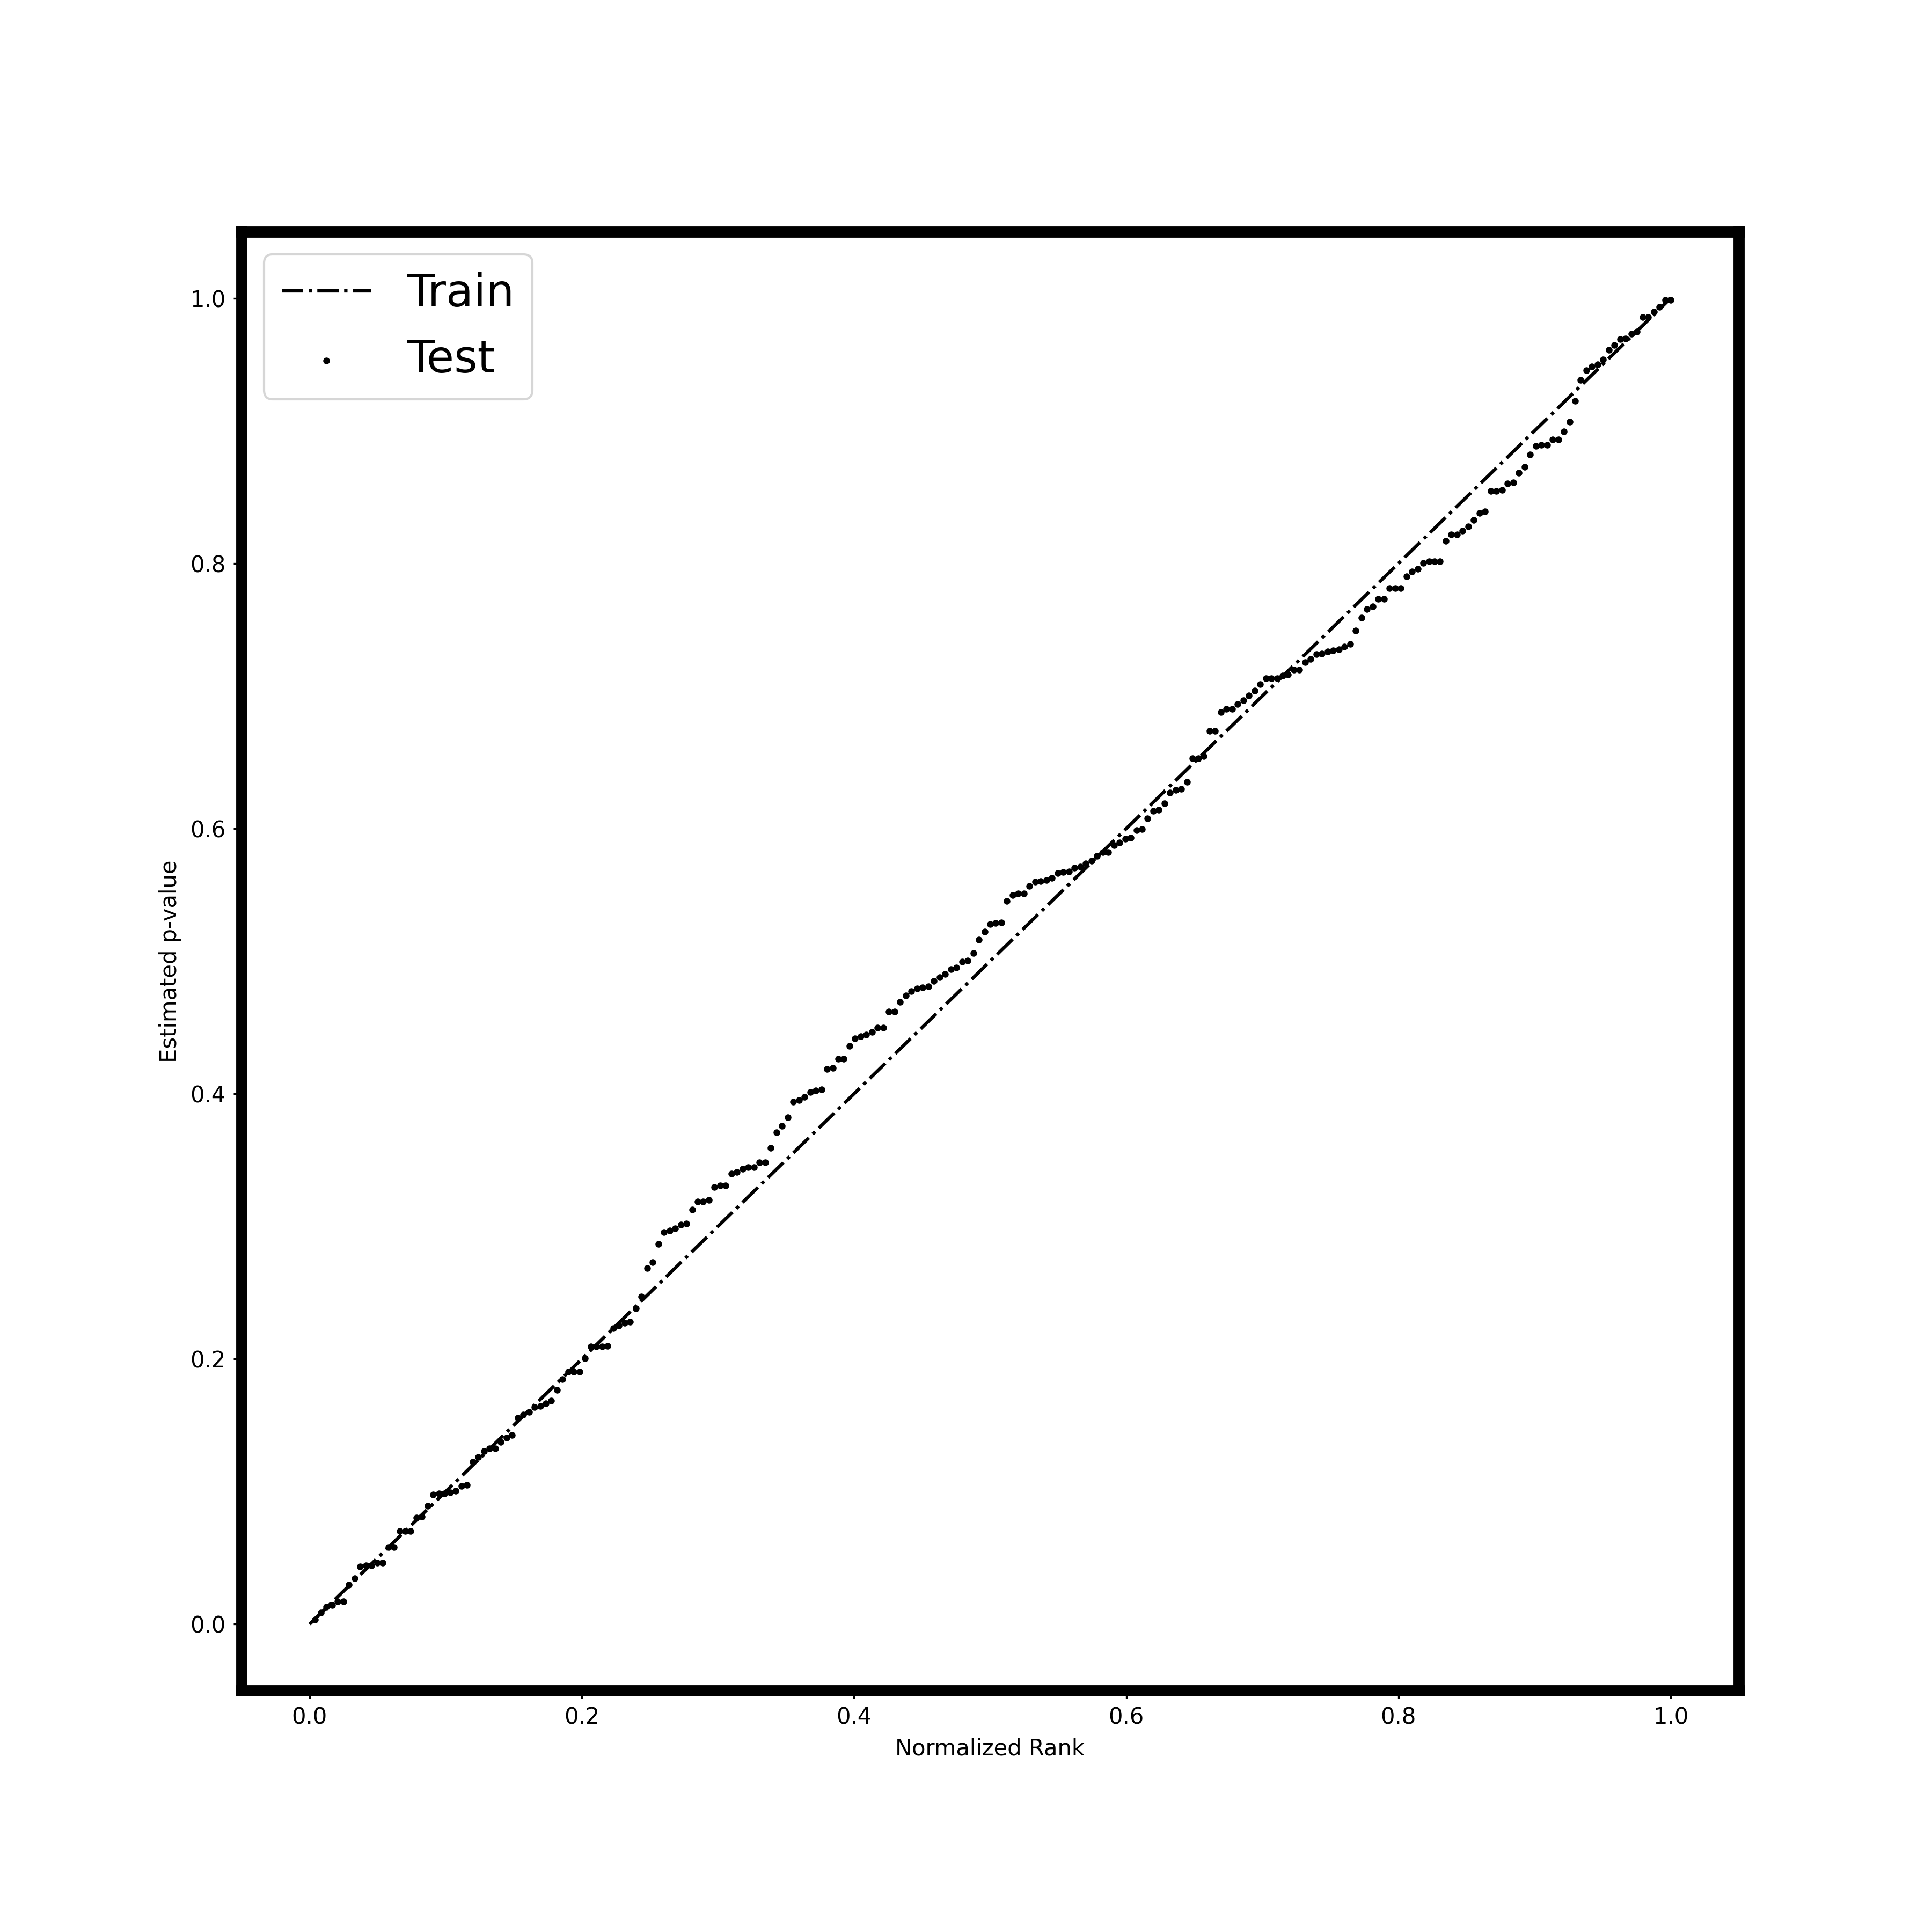
\includegraphics[width=2in]{img/cnn_QQ_multi.png} &
		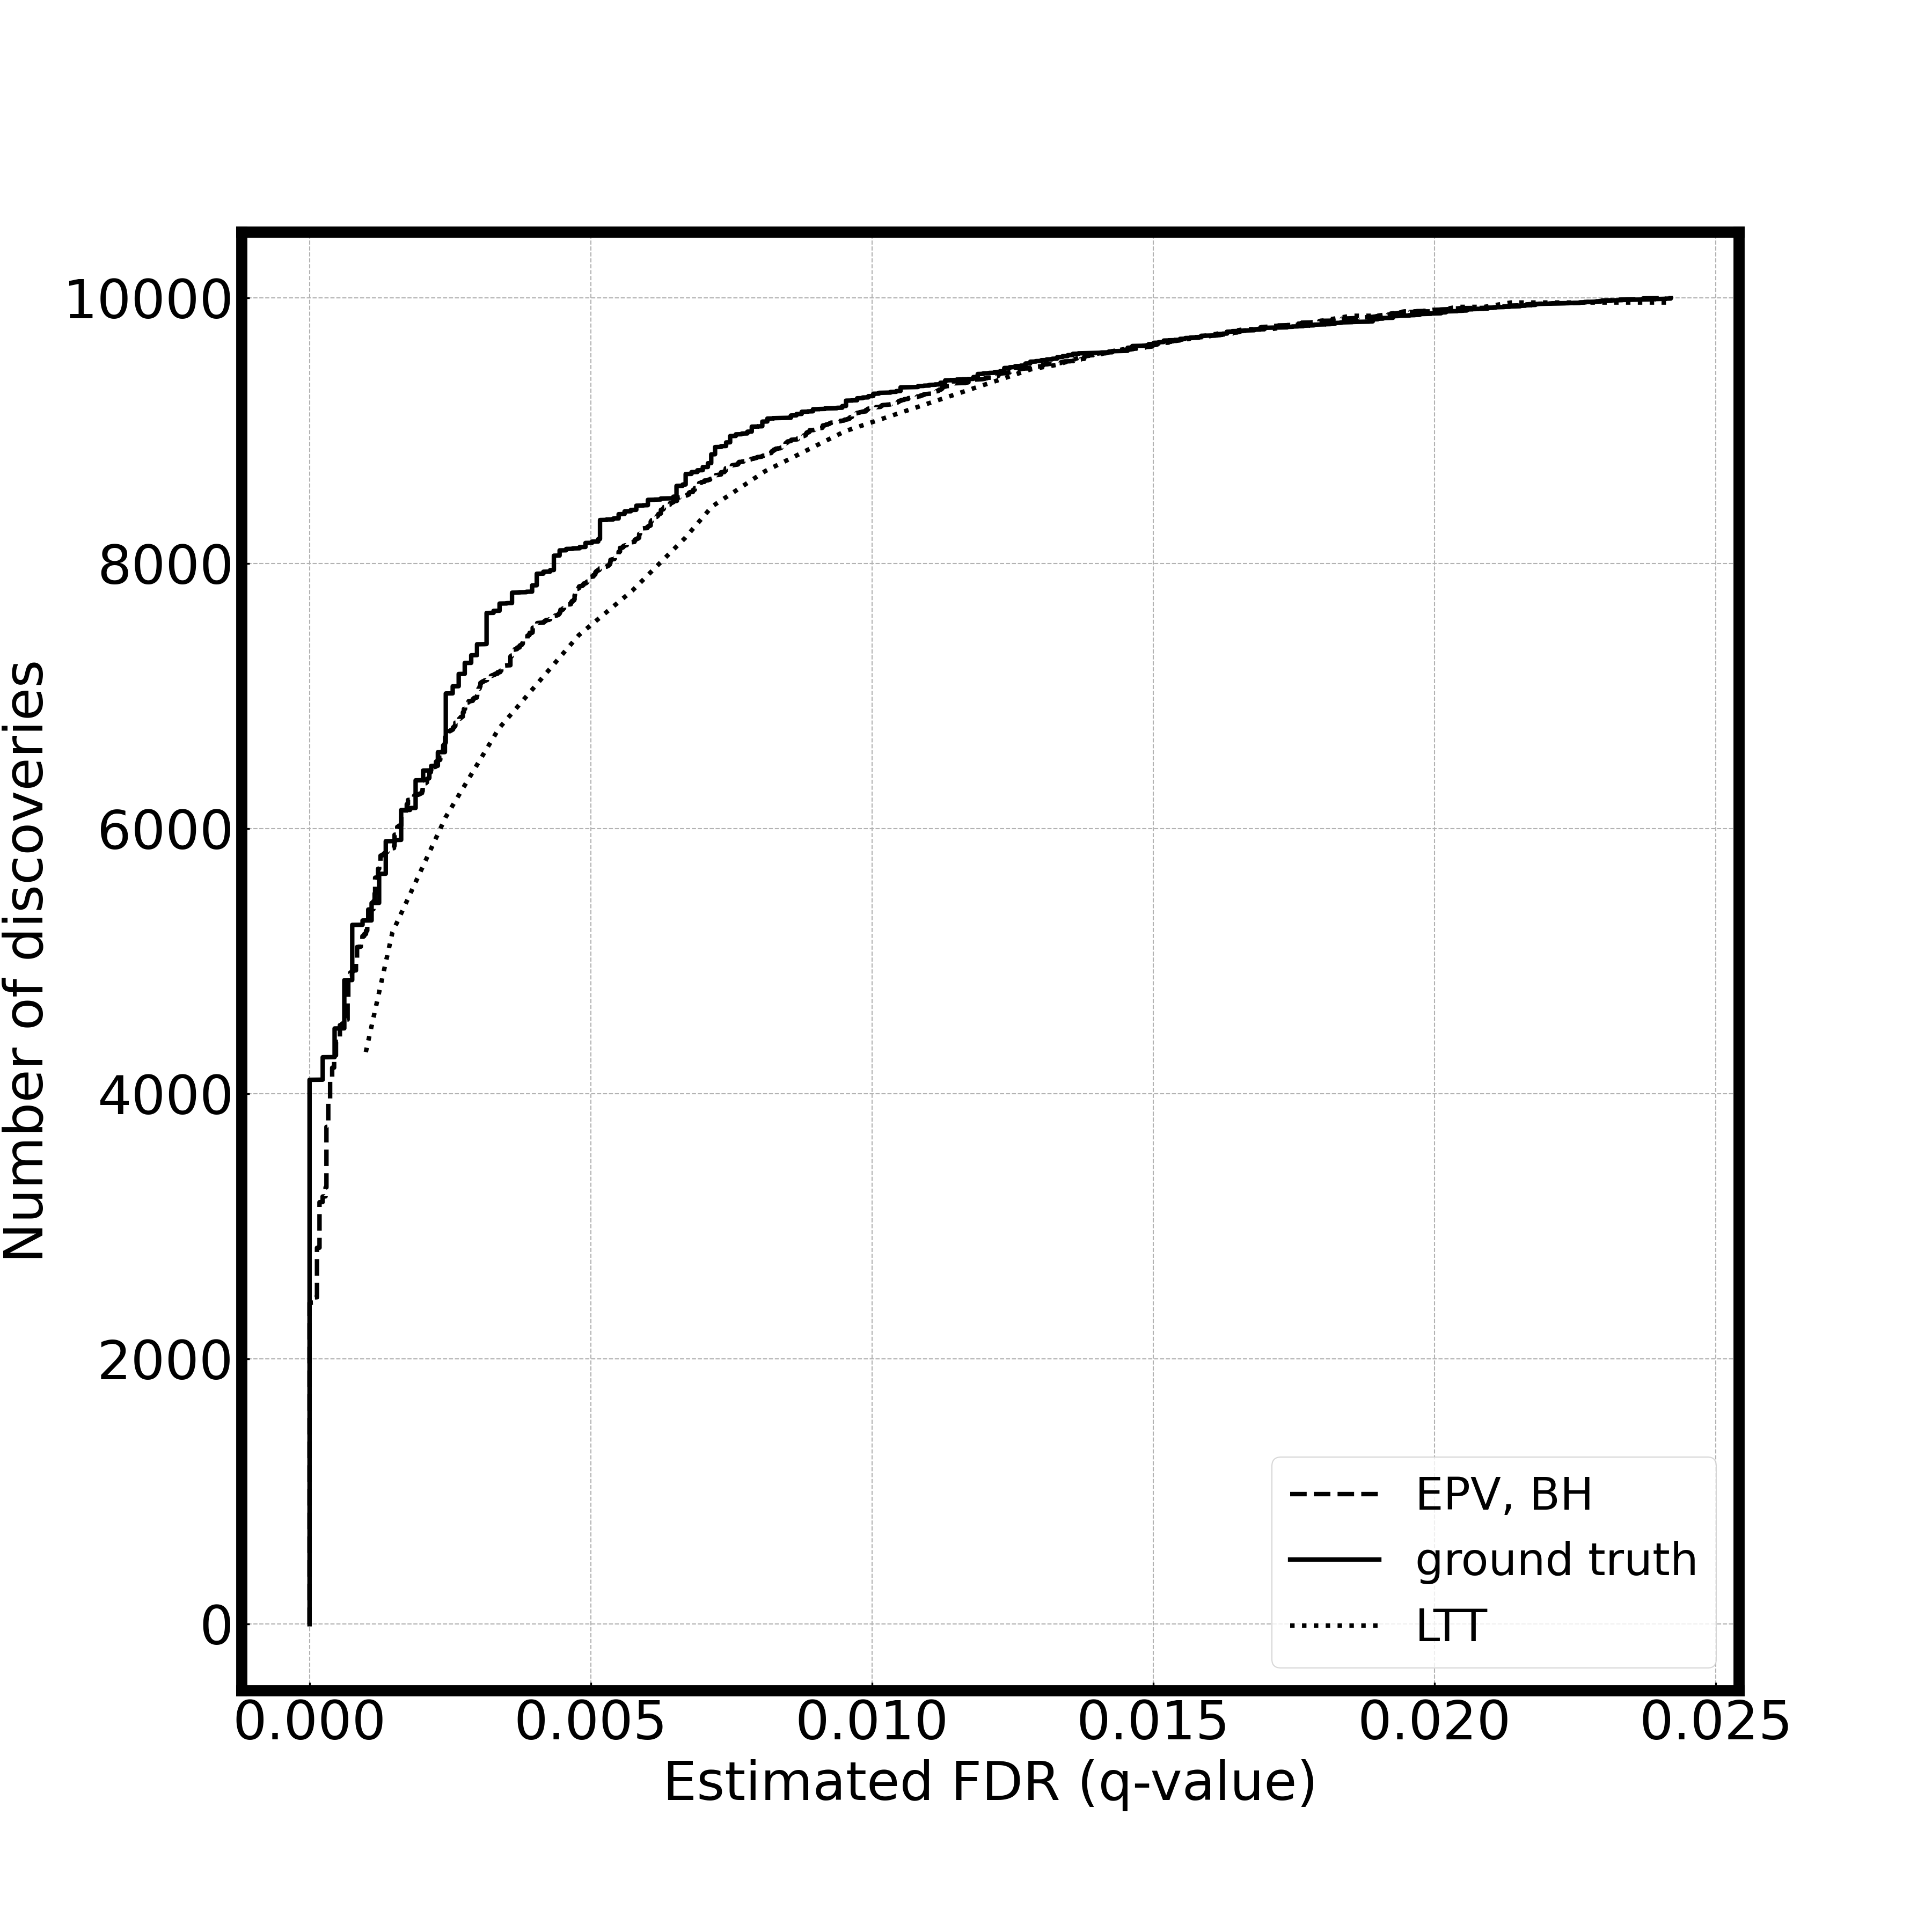
\includegraphics[width=2in]{img/cnn_multi_fdr_control.png}
		\\	
		A & B
	\end{tabular}
	\caption{{\bf  FDR control with p-values for multi-class classification.}
          (A) a QQ plot of the p-values obtained with using negative training data. (B) The number of trusted classifications as a function of the FDR when it is controlled with true labels (black line), with BHP (red line) and LTT (blue line) using the p-values from panel (A).}
	\label{fig:multi}
\end{figure}

Another frequent problem statement is rather a number of classes with only one true label for each sample. In this case we have ten equiprobable classes. The so-called multi-class classification implies getting simultaneously several scores as the model's output. At the same time, EPV approach necessitates separation of scores into negative and positive only. Thus, we insignificantly reformulate our workflow. Here, the p-value indicates the significance that a sample is correctly classified. Consecutively, we work only with the greatest scores among all presented, and the null distribution is constructed from the maximum values for the entire miss-classified training data. Thereby, we aim to control that whether a test data is correctly classified to its class or not. The $\pi_0$, again is estimated by the proportion of the incorrect classification among all samples. It is a tiny number due to the choice of high-performance model in context of resolvable MNIST dataset.

Getting closer to the plots \ref{fig:multi}, we should outline that only two were acquired. Such a situation is still a consequence of CNN superior results, when the error does not exceed several percents. Hence, we could only work with the FDR on a very small range. Nevertheless, a little fall of quality compared to the binary case can be seen on QQ plots. At the same time, EPV still appears to be adjacent to the diagonal at each point with a reasonable maximum distance. If moving to the FDR graph, one can see that this time EPV together with BH protocol noticeably outperform LTT, preserving a high level of interpretability as a smoother version of ground truth.


\begin{figure}
    \centering
        \begin{tabular}{ccc}
 		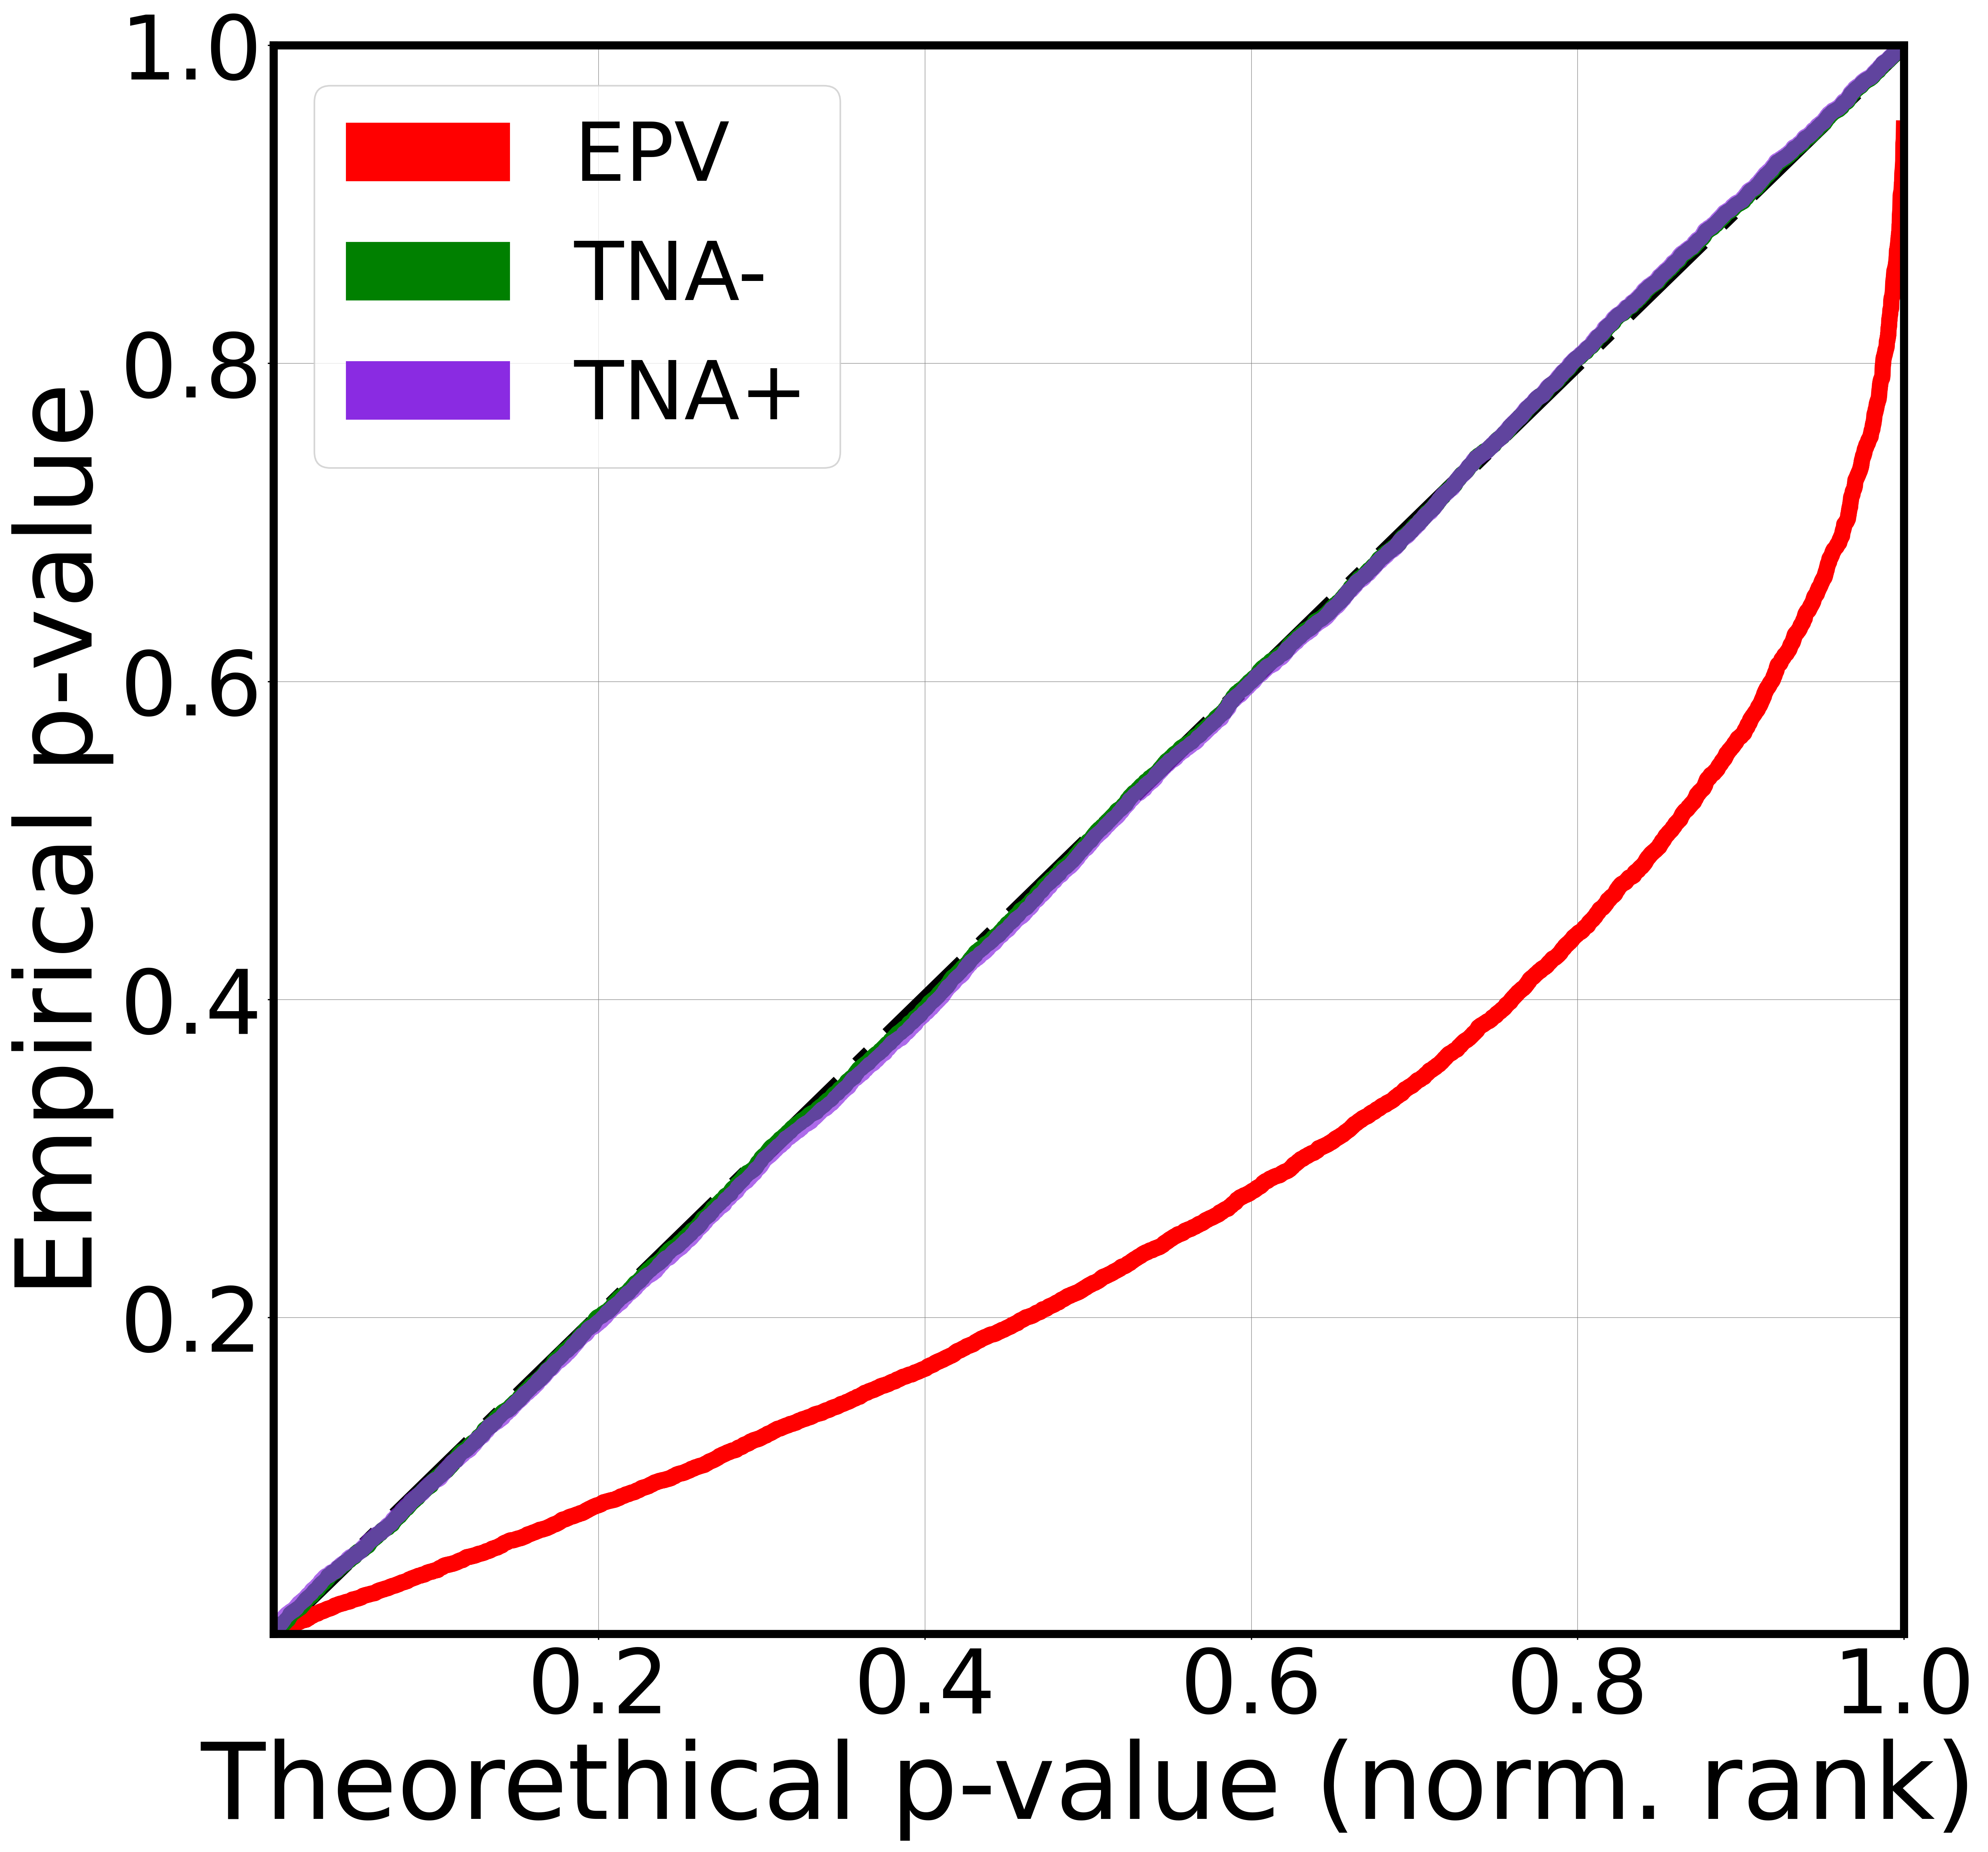
\includegraphics[width=2in]{img/cnn_QQ_shifted.png} &
		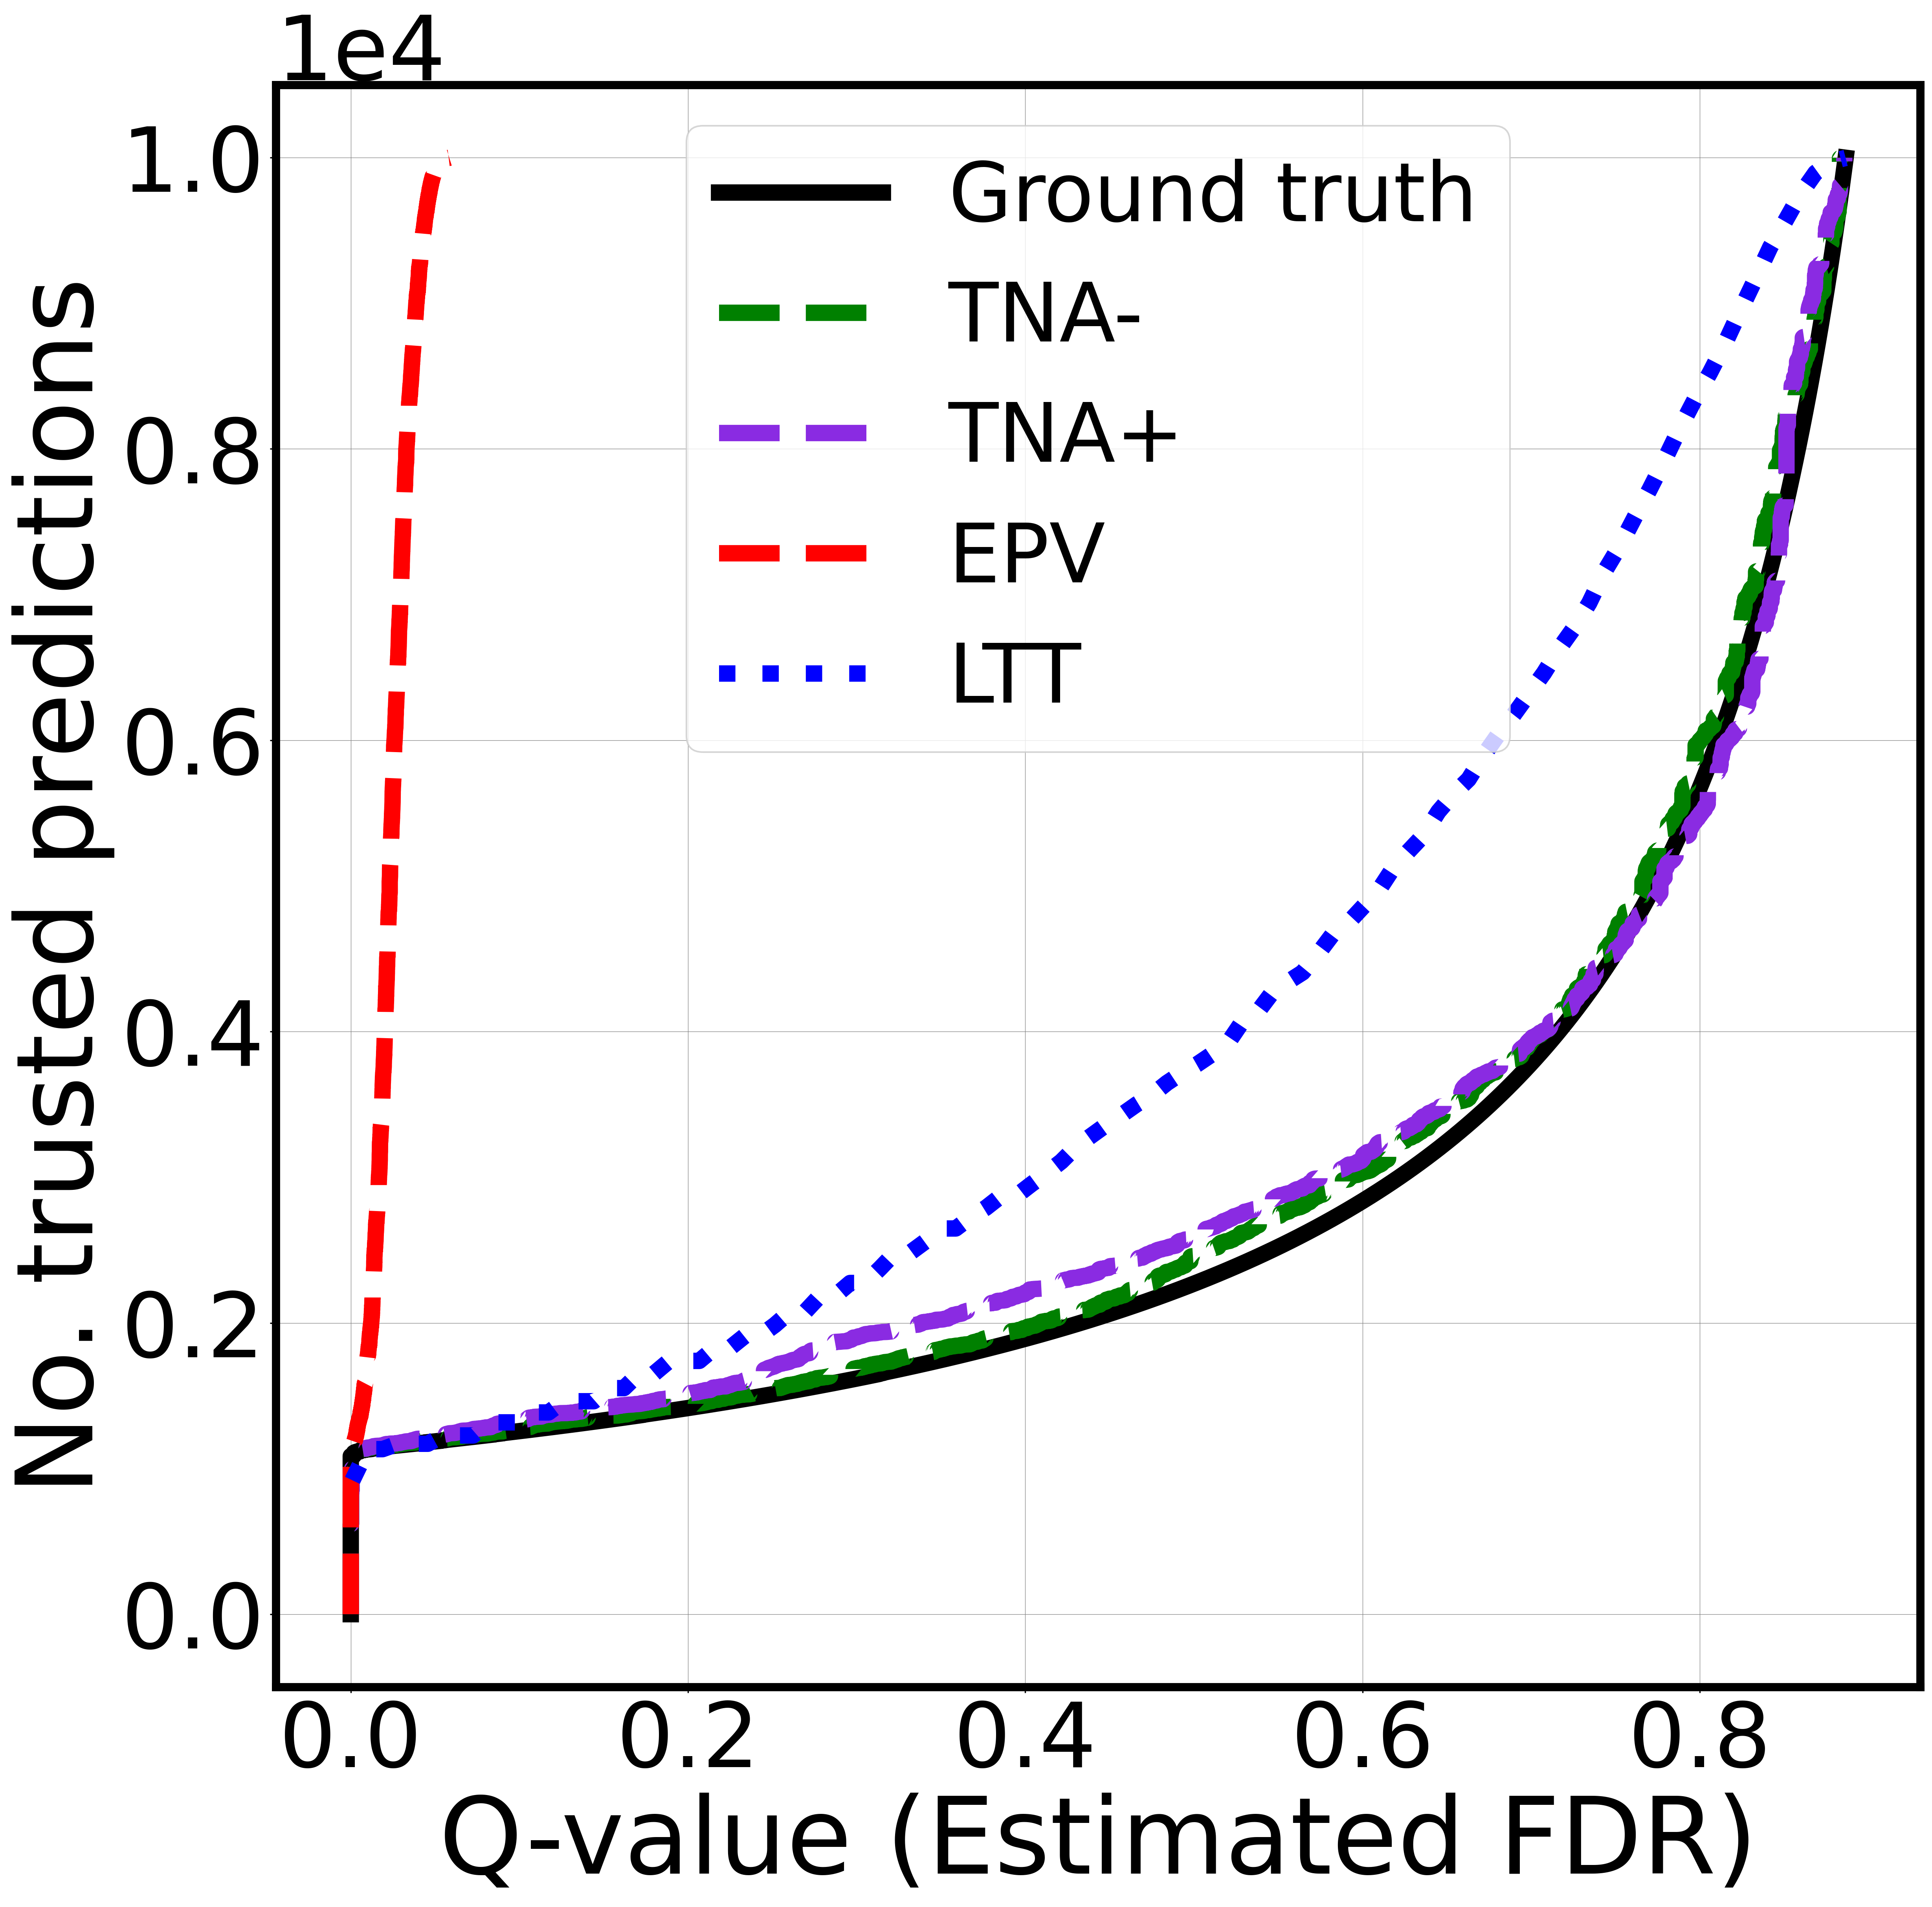
\includegraphics[width=2in]{img/cnn_shifted_fdr_control.png} & 
            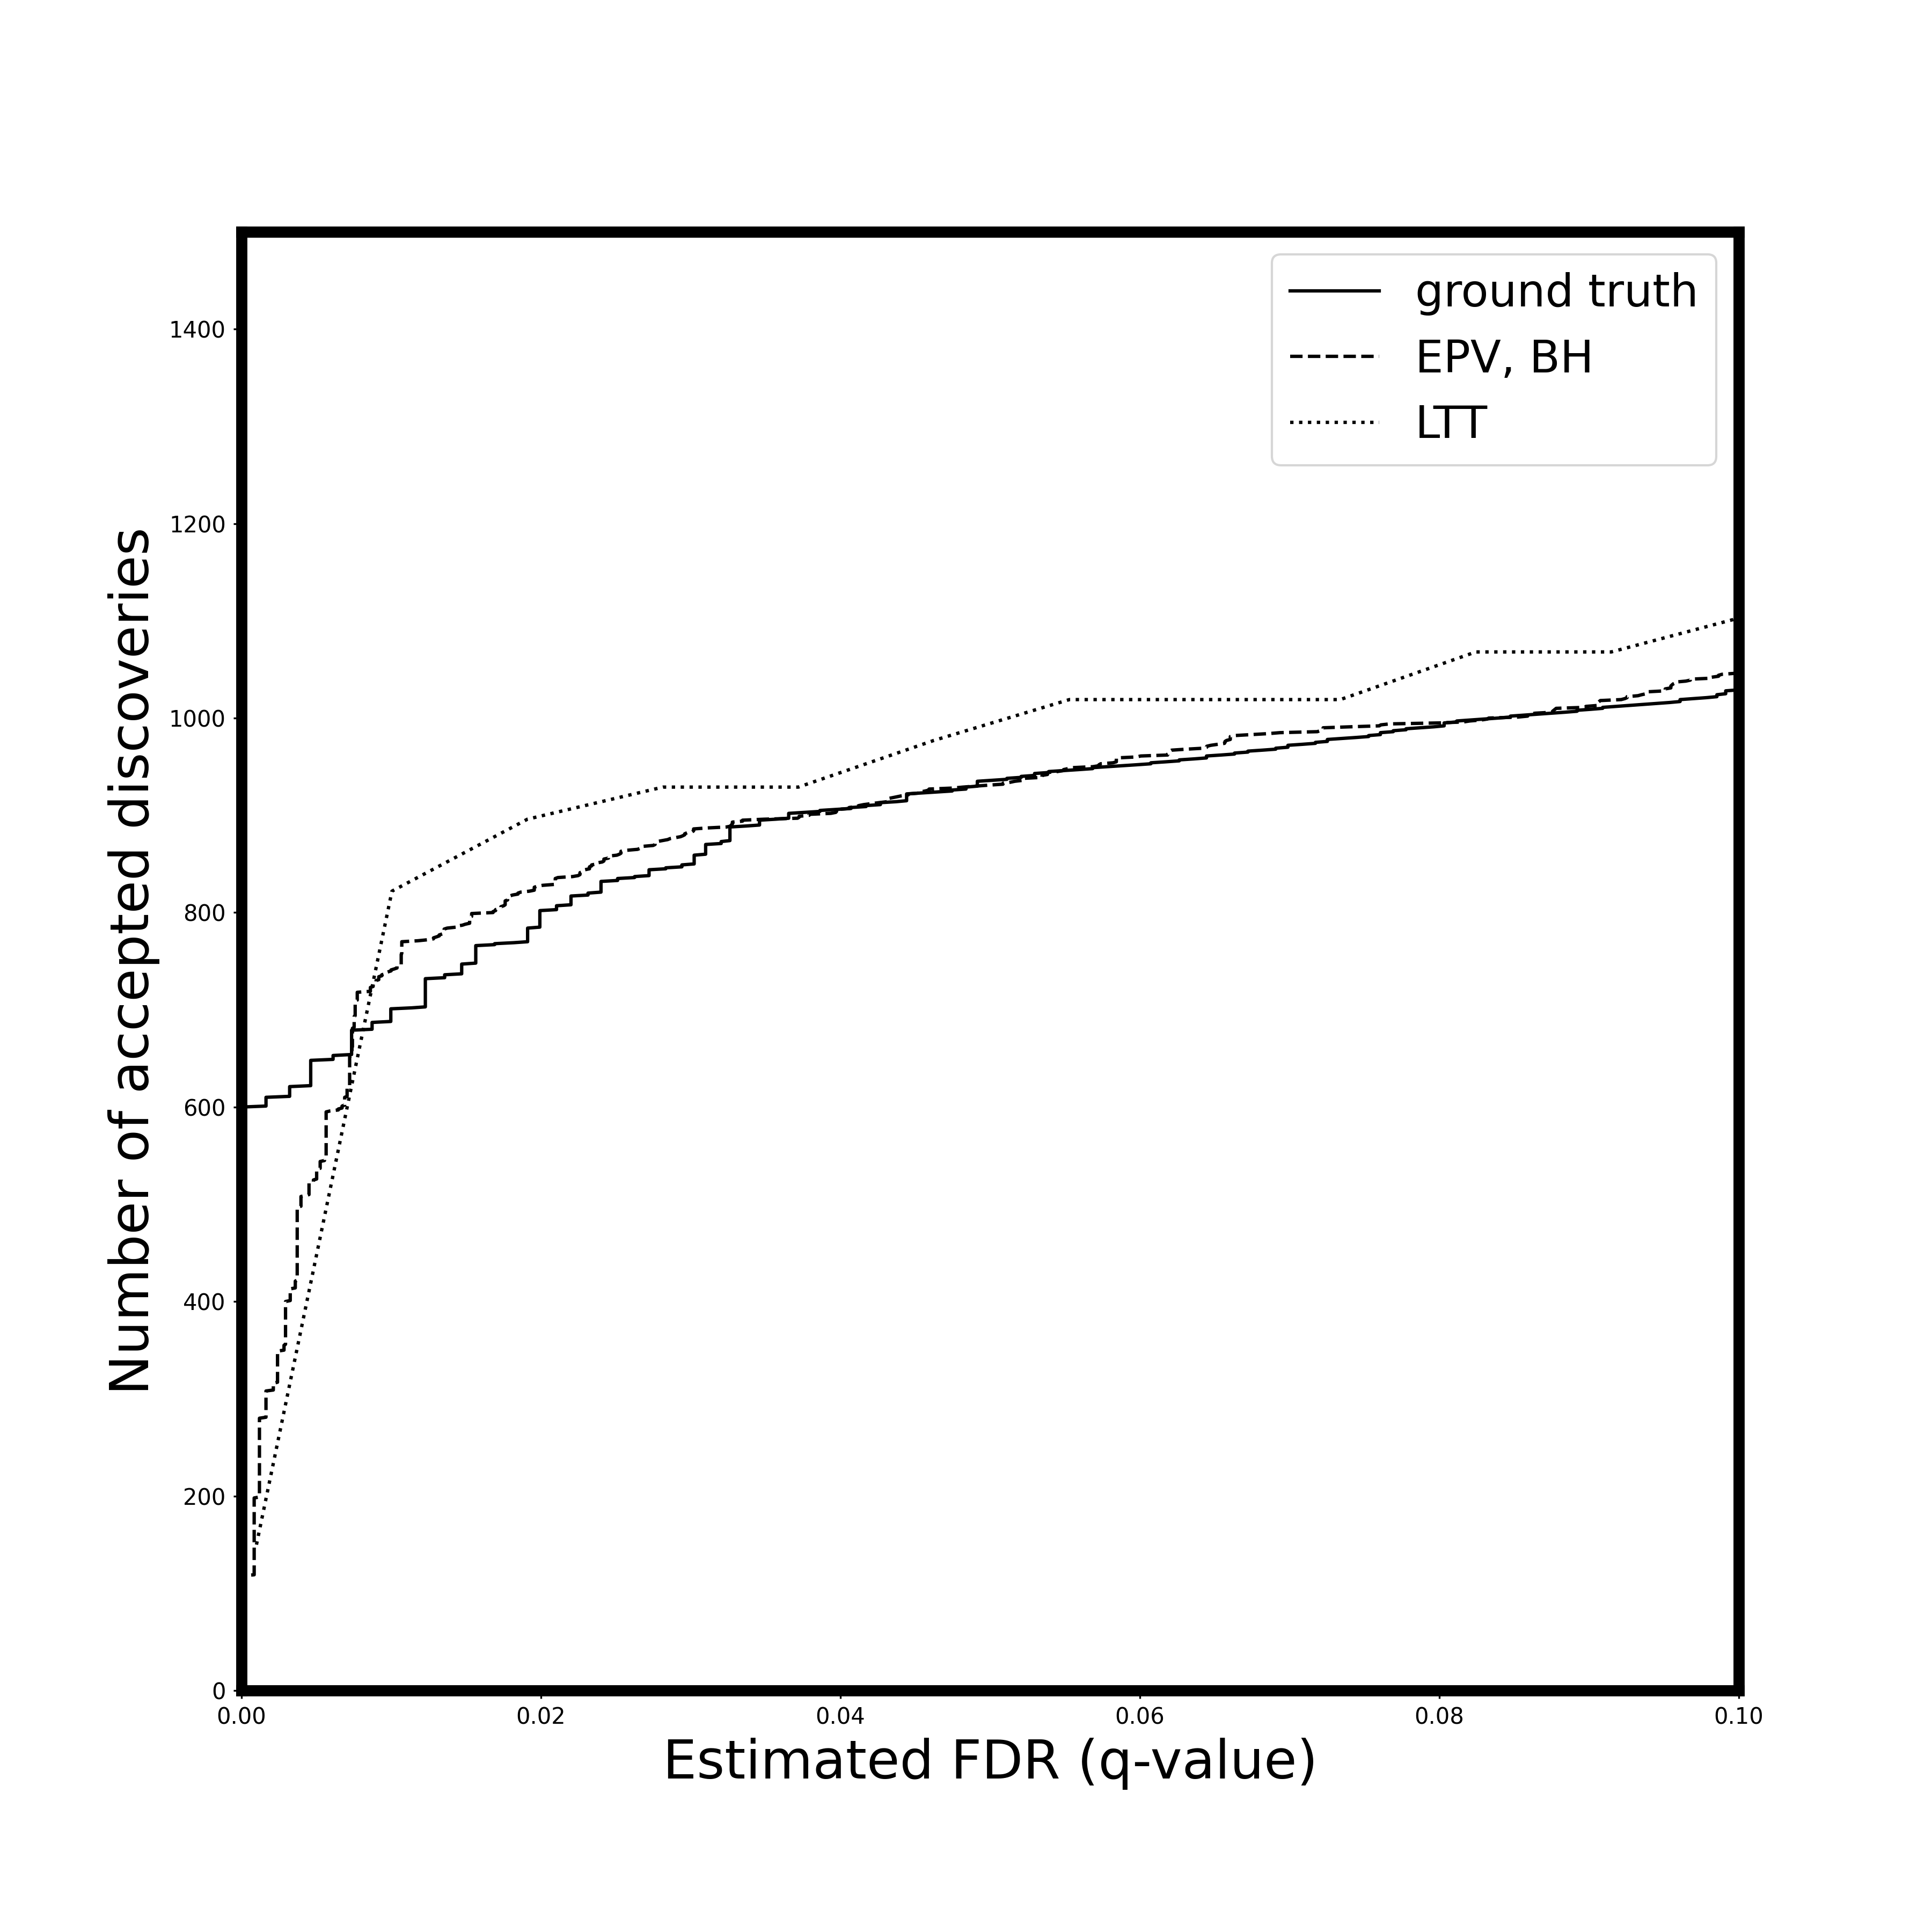
\includegraphics[width=2in]{img/cnn_shifted_fdr_control_loc.png}
		\\	
		A & B & C
	\end{tabular}
	\caption{{\bf  FDR control with p-values for detecting data distribution shift.}
		(A) a QQ plot of the p-values obtained with using negative training data. (B) The number of trusted classifications as a function of the FDR when it is controlled with true labels (red line) and with controlled with BHP (black line) using the p-values from panel (A).
		(A) a QQ plot of the p-values obtained with using training data classified as negative. (B) The same as panel (B), but using p-values from panel (C).
	}
	\label{fig:shift}
\end{figure}

\subsection{Shift case}

As it was declared, MNIST has a set of properties, making it restricted for a comprehensive analysis. For instance, it does not allow to check wherever methods are resilient to shifts in data distribution. Therefore, we trained the CNN on described binary task with preserved target label "2". However, for further examination of p-values’ nature, we introduce a 1-by-1 southeast pixel move for each test image. The newly born samples with shifted data distribution depict such a scenario, when upcoming test data has a visible difference from the training phase. 

\begin{figure}
    \centering
        \begin{tabular}{c}
 		A. Positive samples \\ 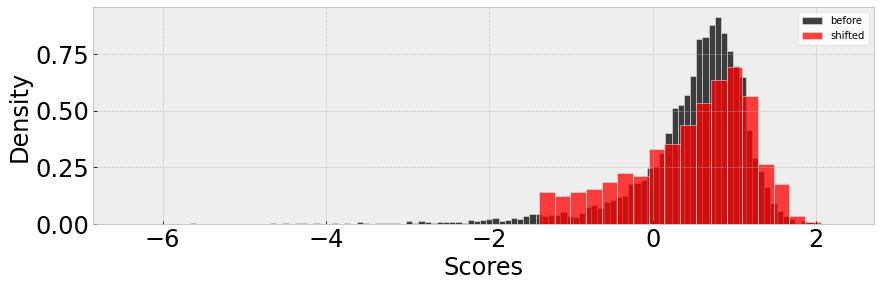
\includegraphics[width=6in]{img/shift_score_pos.png} \\
		B. Negative samples \\ 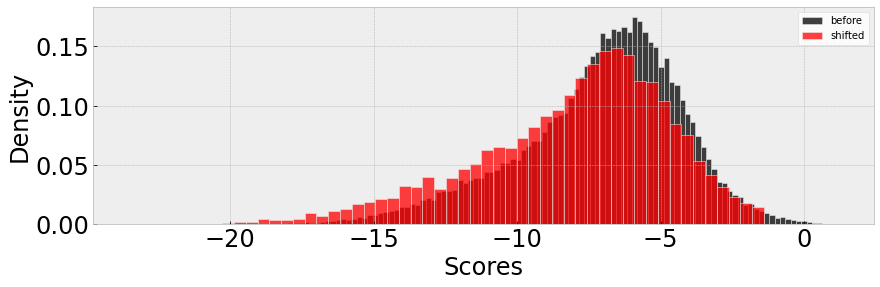
\includegraphics[width=6in]{img/shift_score_neg.png}
	\end{tabular}
	\caption{{\bf   Model's scores before and after shift in test data distribution.}
        (A) a score distribution of positive test samples according to predictions, where the black color stands for the normal case and the red one - for the shifted case. (B) has identical meaning to panel (A), except for the usage of negative samples.}
	\label{fig:scores}
\end{figure}

So, the final part of the experiment implies running the altered images through the already trained model. On the resulting graphs \ref{fig:shift}, we would identify the first perceptible limitation of our EPV methodology if eliminating the statistical part with $\mu$ and $\sigma$. Nevertheless, the stated methodology keeps maintaining a notable proximity to the ground truth plot in terms of the long run. However, the local range depicts a downward shift. At the same time, LTT, also experiencing difficulties, again shows ubiquitously worse results. Another evidence of EPV's consistency in case of data shifts is depicted on the QQ plot, where the test dots do not make any sufficient drift from the diagonal. 

The reason for such a behavior is that for our particular experiment's environment a shift can be identified not only in data distribution, but also in scores distribution (shown on \ref{fig:scores}). The left boundary of the initial shifted test results has made a serious leftwards move, meaning far more test cases started obtaining a unit p-value (1.0). This is the reason why our EPV algorithm demands statistical unification of test and train data, separated by positive and negative sets.

\subsection{Balanced case}


\begin{figure}
    \centering
        \begin{tabular}{ccc}
 		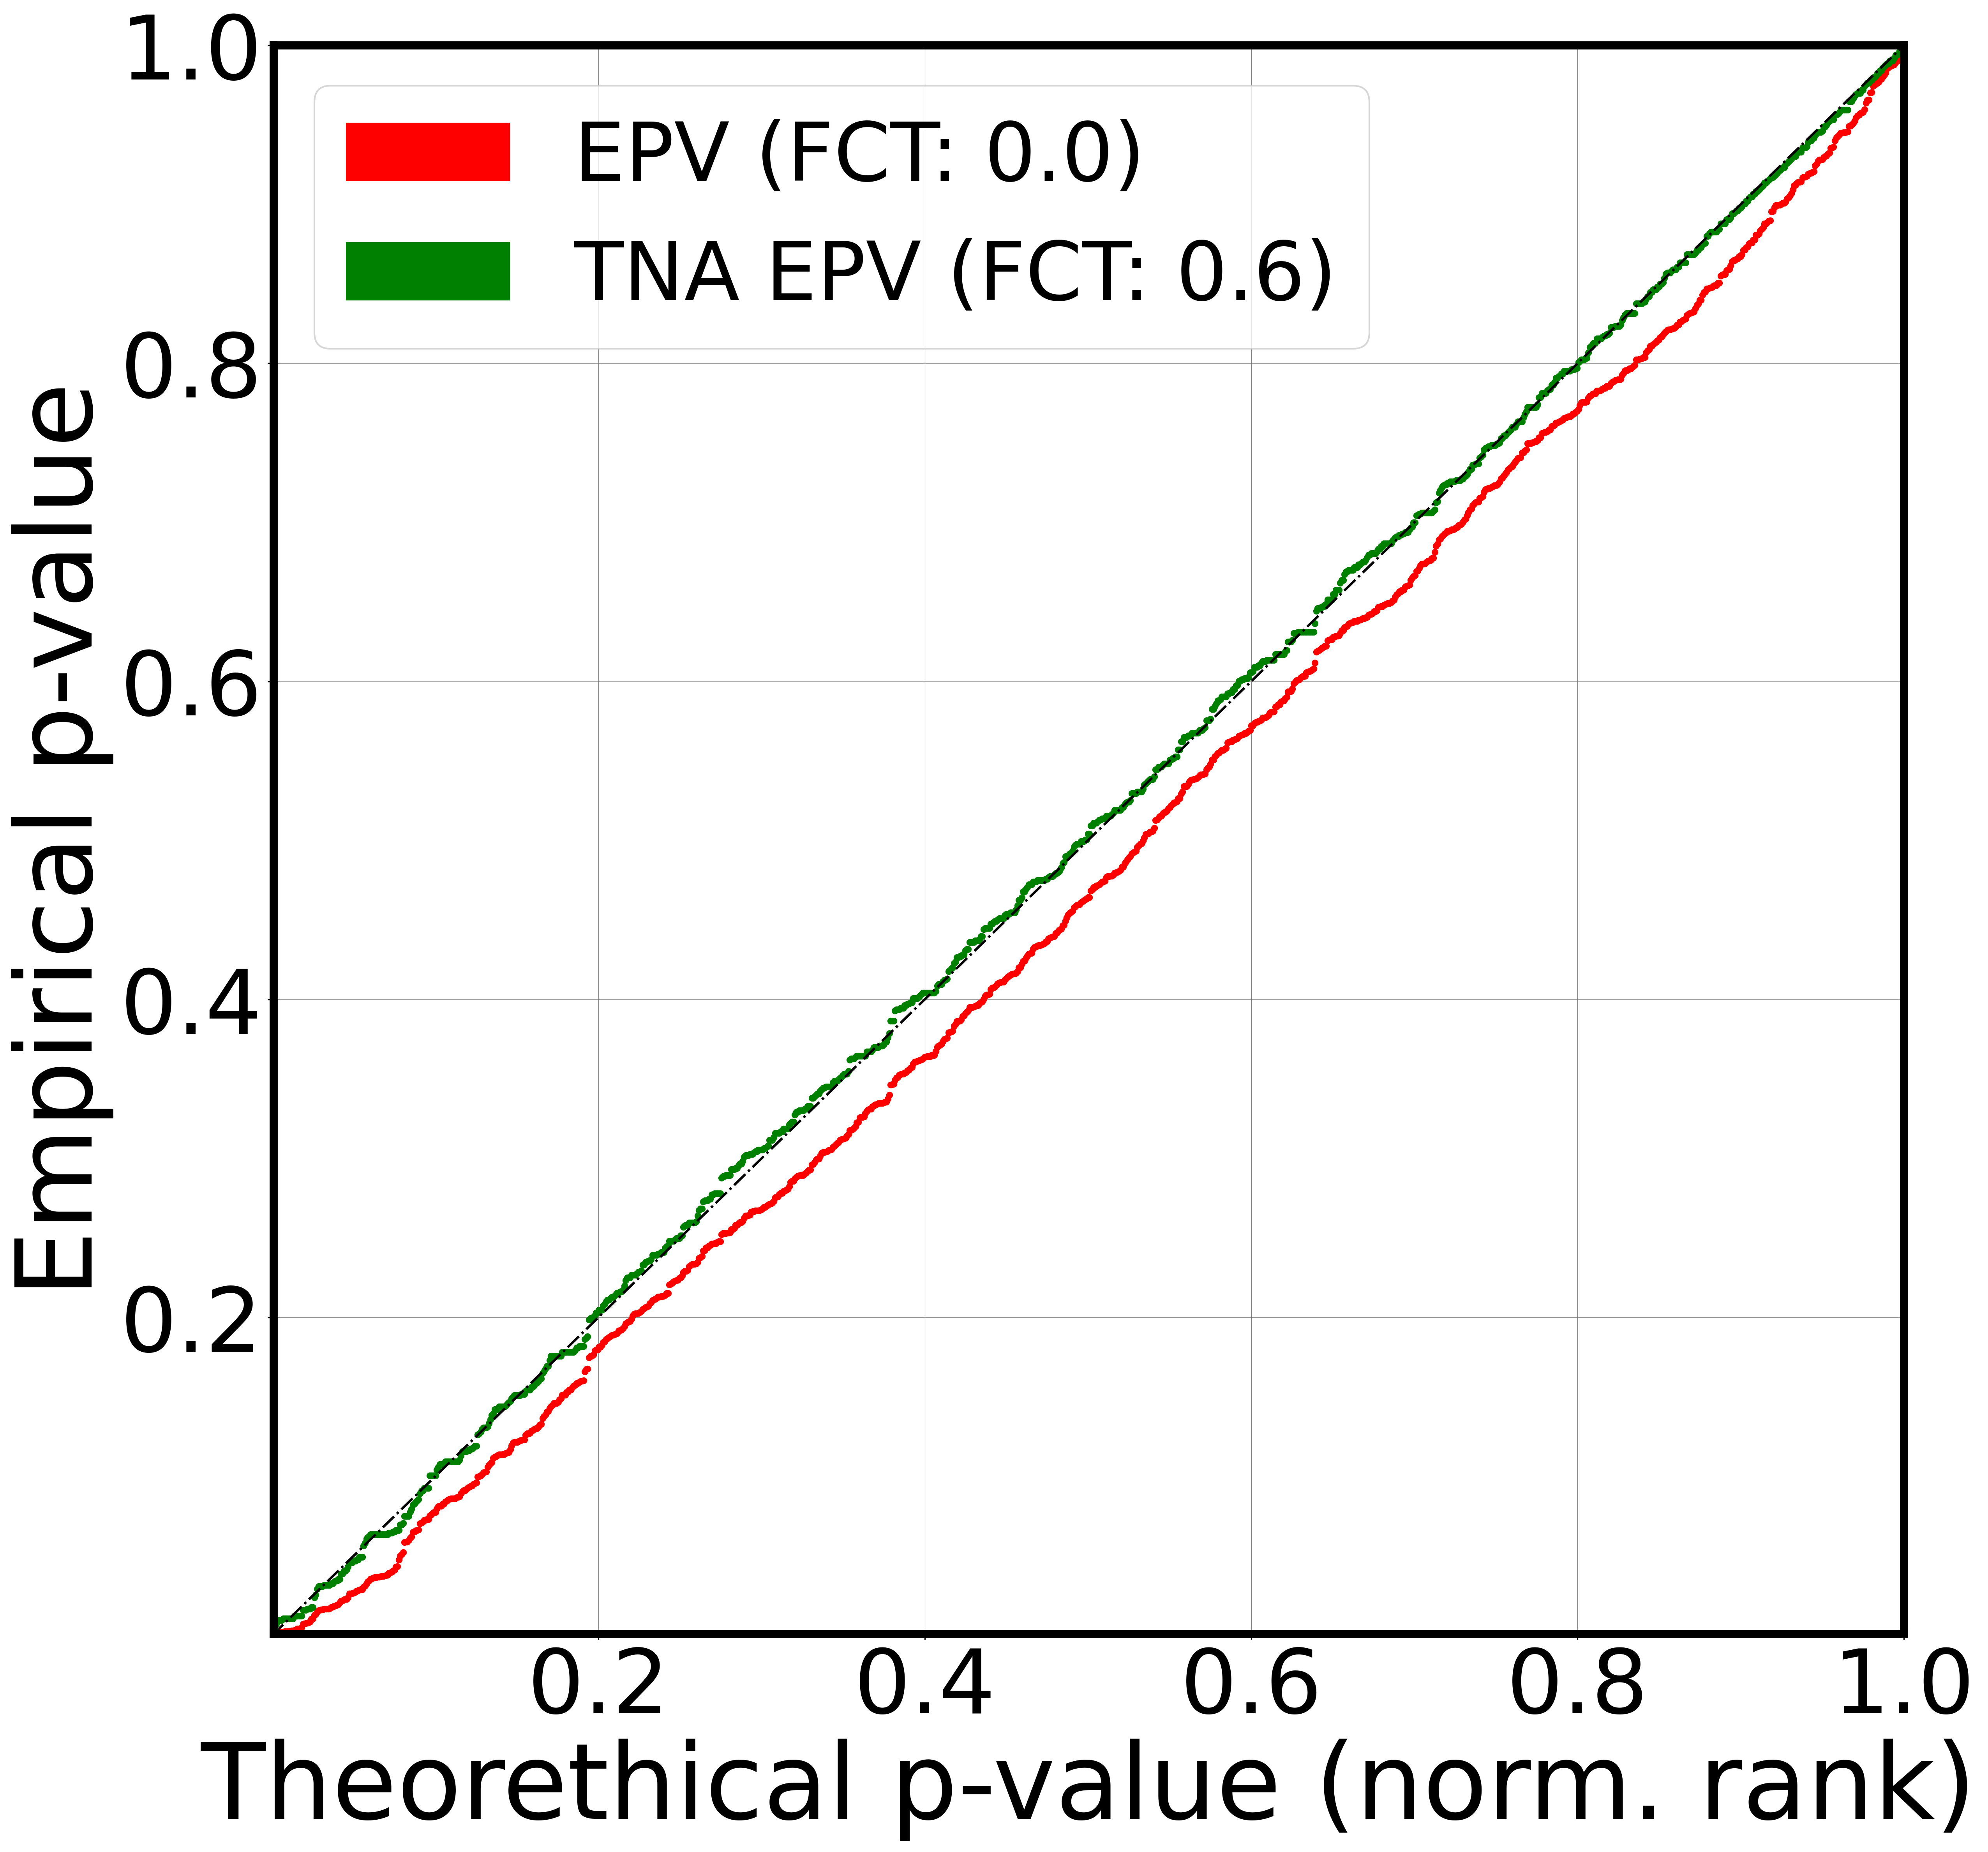
\includegraphics[width=2in]{img/cnn_QQ_balanced.png} &
		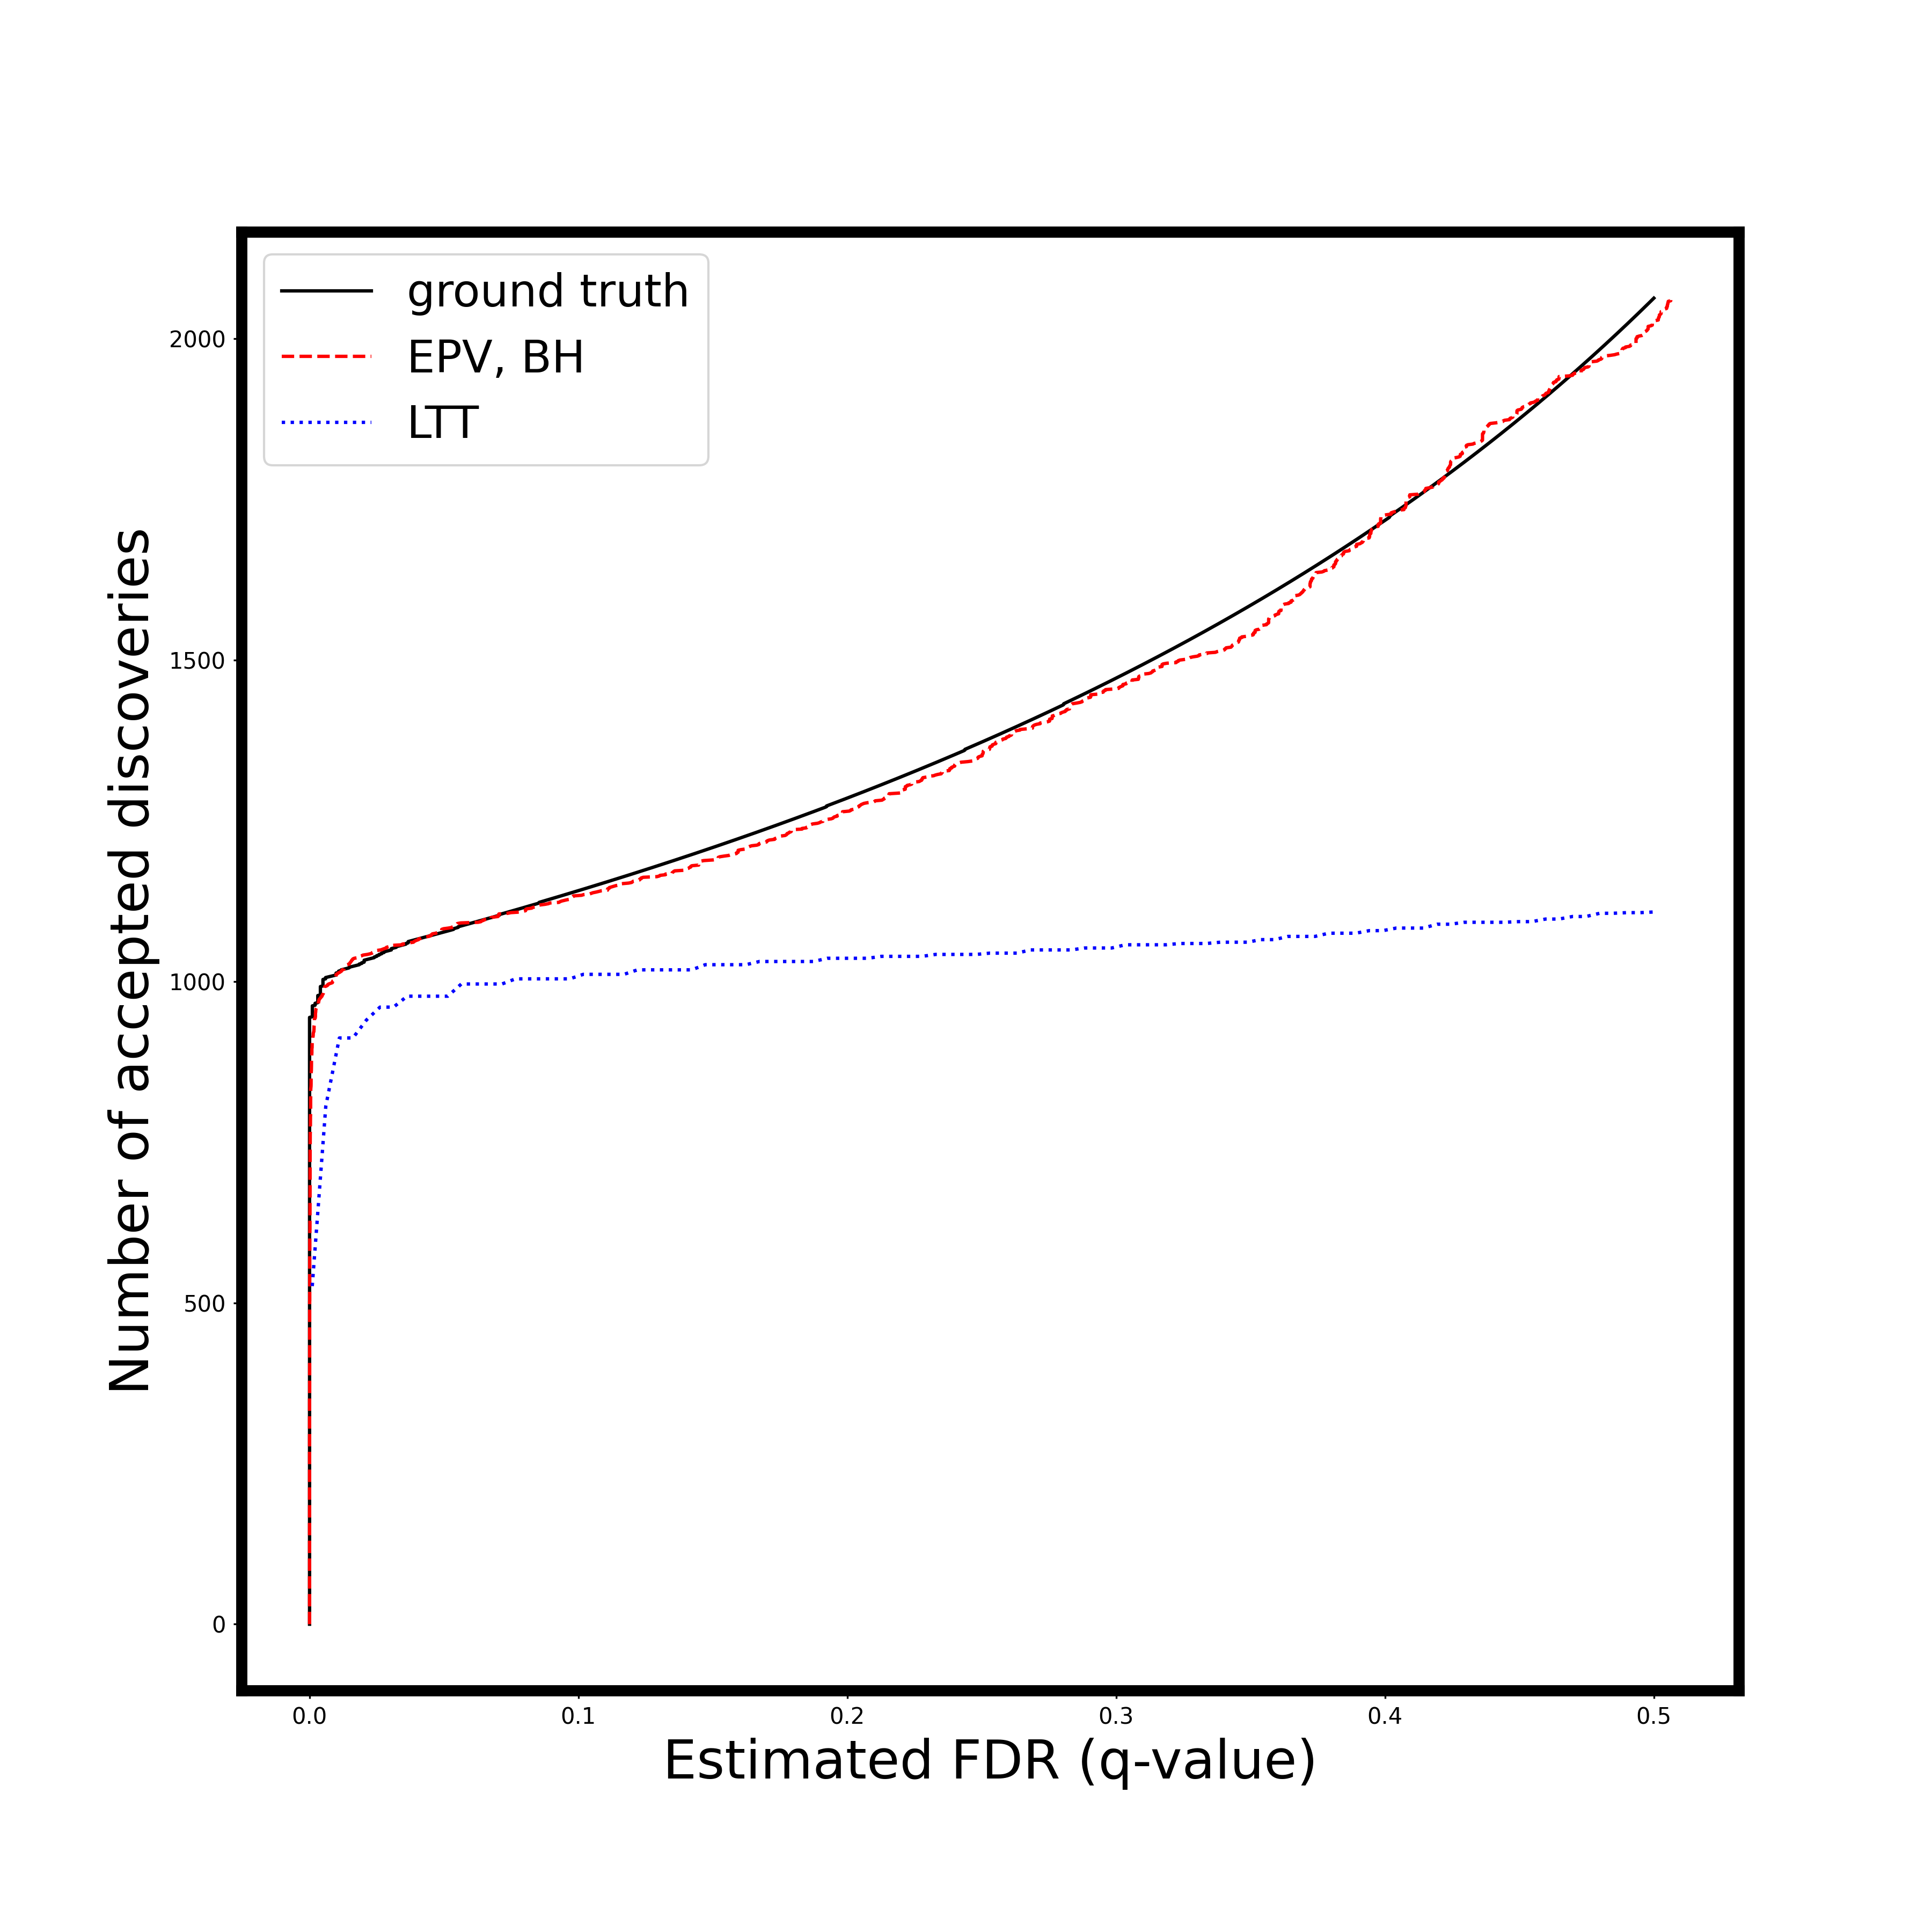
\includegraphics[width=2in]{img/cnn_balanced_fdr_control.png} & 
		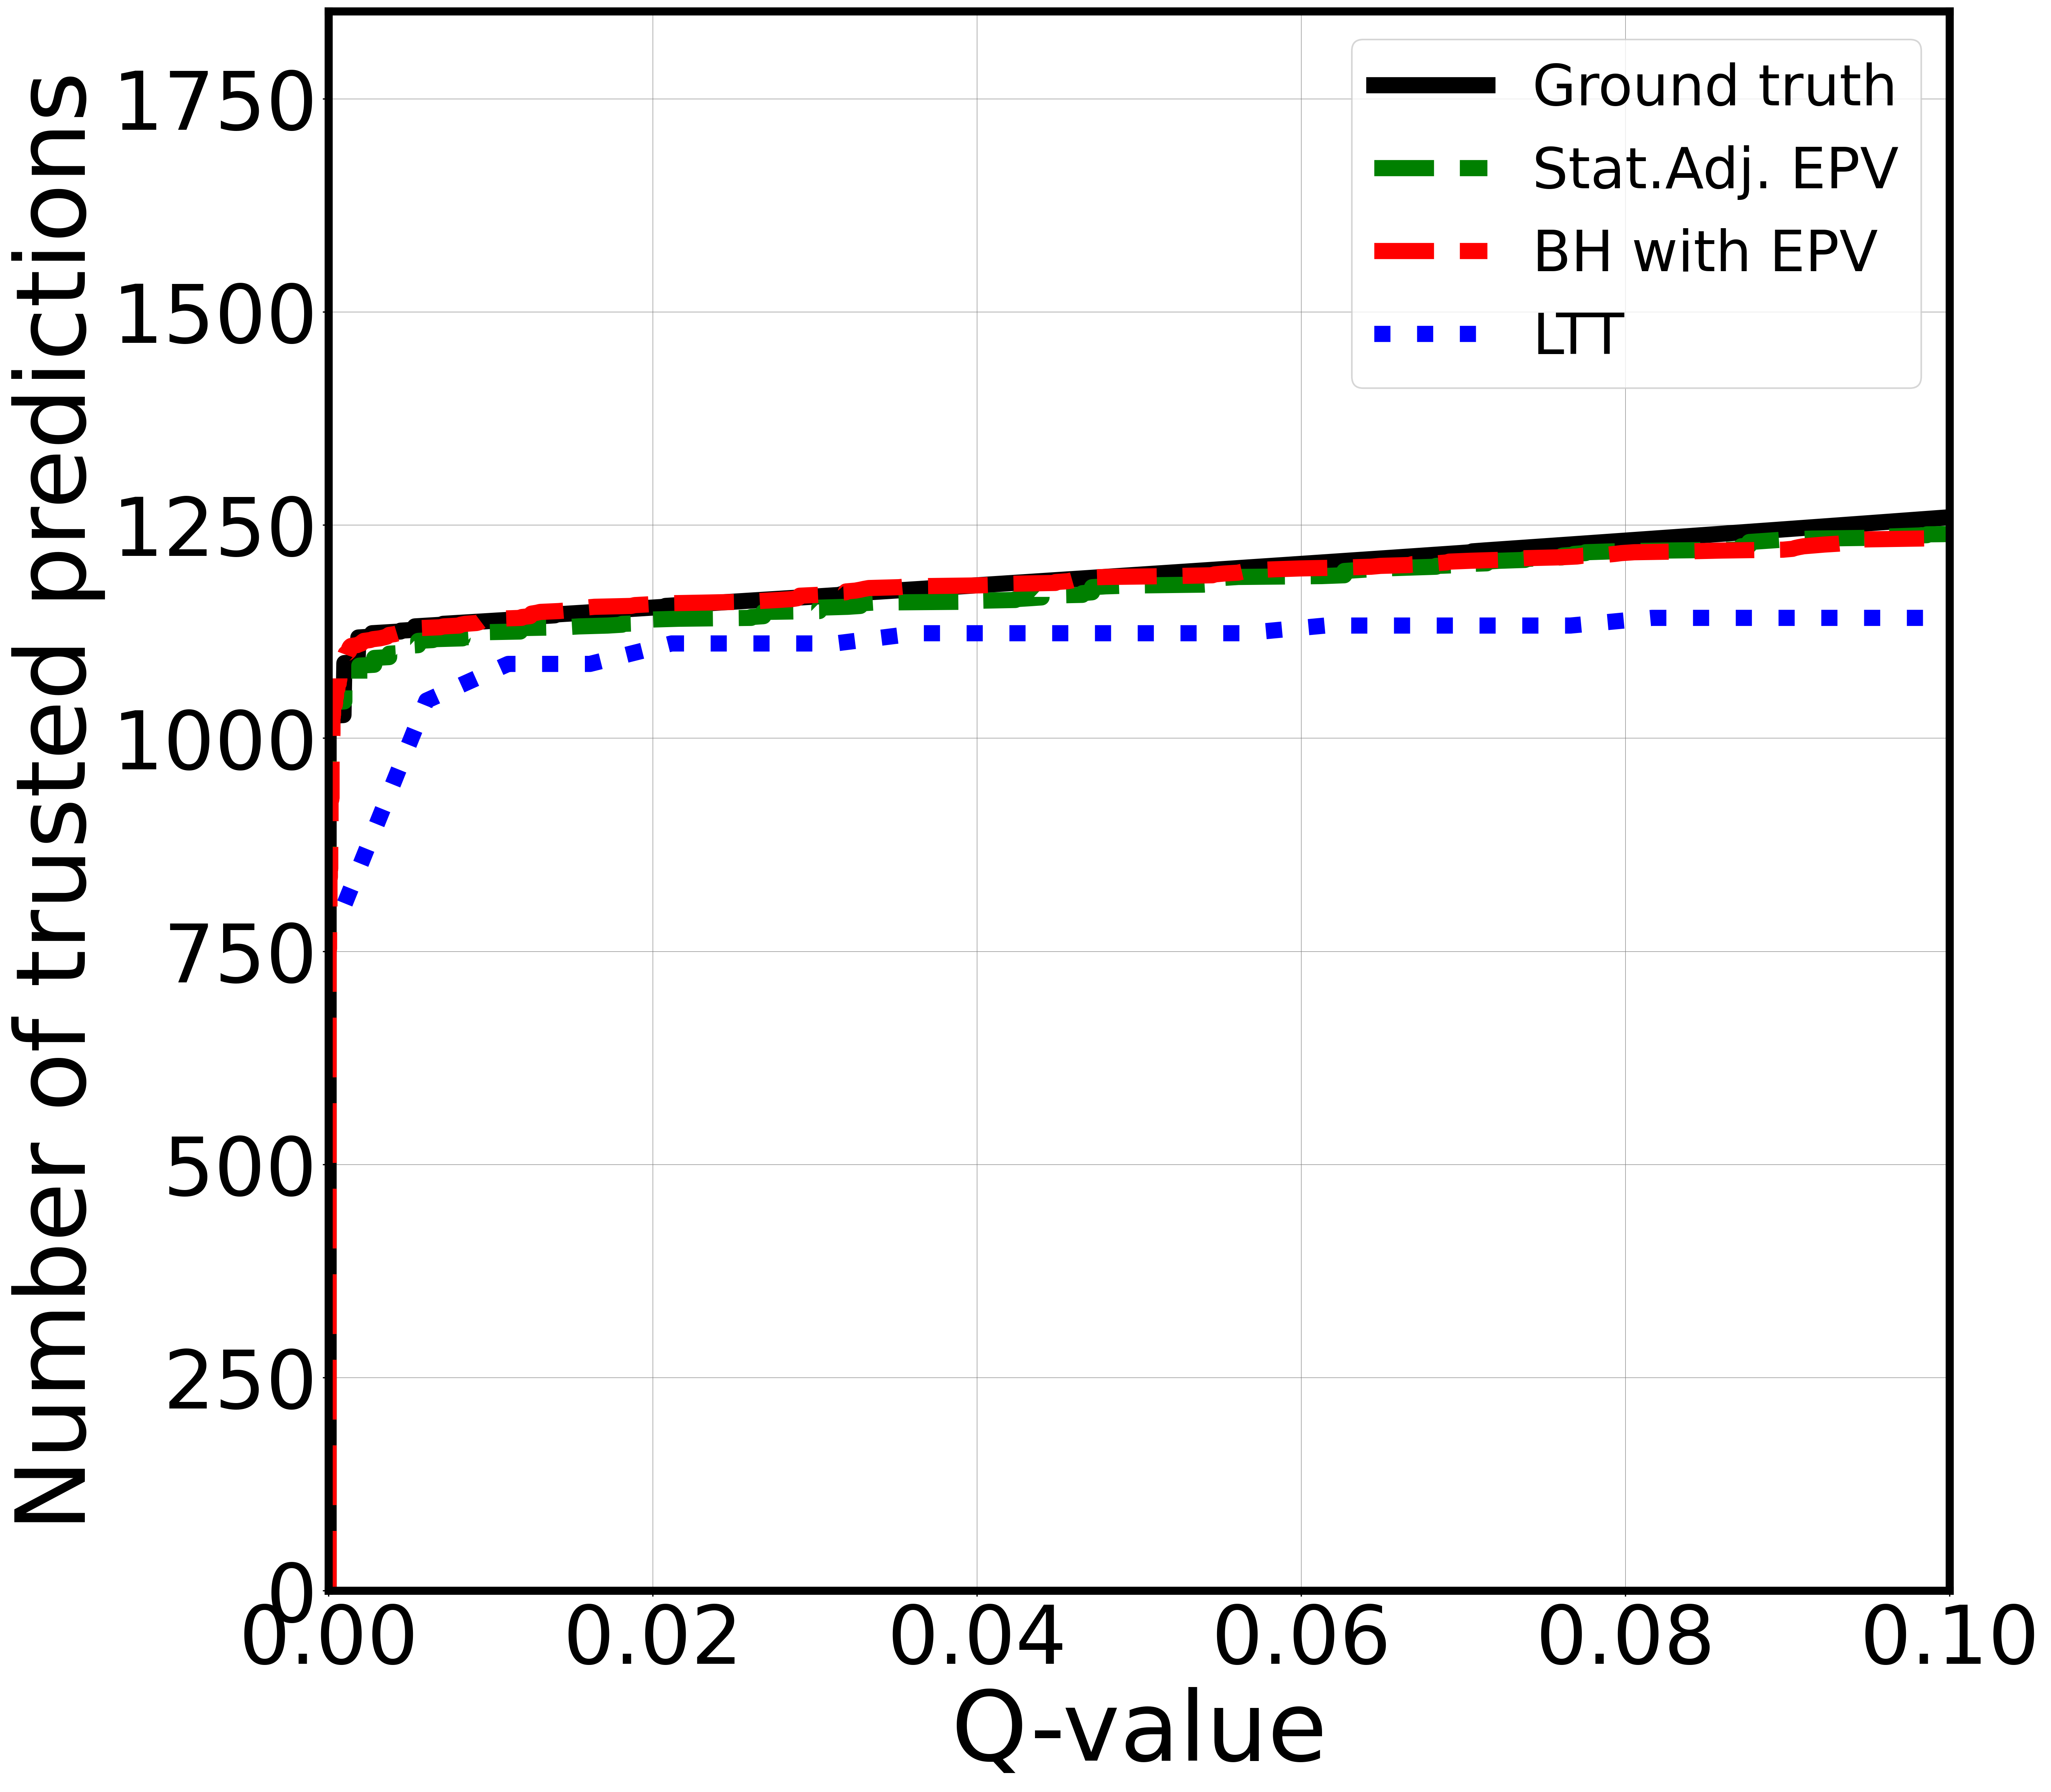
\includegraphics[width=2in]{img/cnn_balanced_fdr_control_loc.png}
		\\	
		A & B & C
	\end{tabular}
	\caption{{\bf  FDR control with p-values for altered class proportions.}
        (A) a QQ plot of the p-values obtained with using negative training data. (B) The number of trusted classifications as a function of the FDR when it is controlled with true labels (black line), with BHP (red line) and LTT (blue line) using the p-values from panel (A).
        (C) corresponds to the local range of graph (B).}
	\label{fig:balanced}
\end{figure}

Final conditions to be described imply another form of dataset's alteration. However, this time the proportion of positive and negative classes is changed rather than the data itself. Instead of inferring on the entire available test dataset, we collect all the positive samples (composing only 10 percent) and append the equal amount of negative samples in accordance with true labels for the sake of experiment's requirements. The declared parity differs from the share of classes, which the model has seen during training. Hence, a highly probable real-life scenario is tested here.

Again, straightforward implementation of EPV without any statistical corrections was leading to the low algorithm's ability to describe the ground truth. However, transferring the entire approach into the current form made a drastic amelioration. As it can be seen on figure \ref{fig:balanced}, our method plus BH protocol work almost perfectly, with a little bit higher number of discoveries predicted on the local range. On the contrary, the LTT framework, based on FWER-family approach, shows comparatively dreary results, behaving illogically in terms of ground truth. If moving to the \ref{fig:balanced}A, we can see ultimately close scatter plot to the "Train" diagonal.

\section{Discussion}

\subsection{Proving statistical adjustment}

\begin{figure}
    \centering
        \begin{tabular}{ccc}
 		
\includegraphics[width=2in]{img/good_QQQ.png} &
		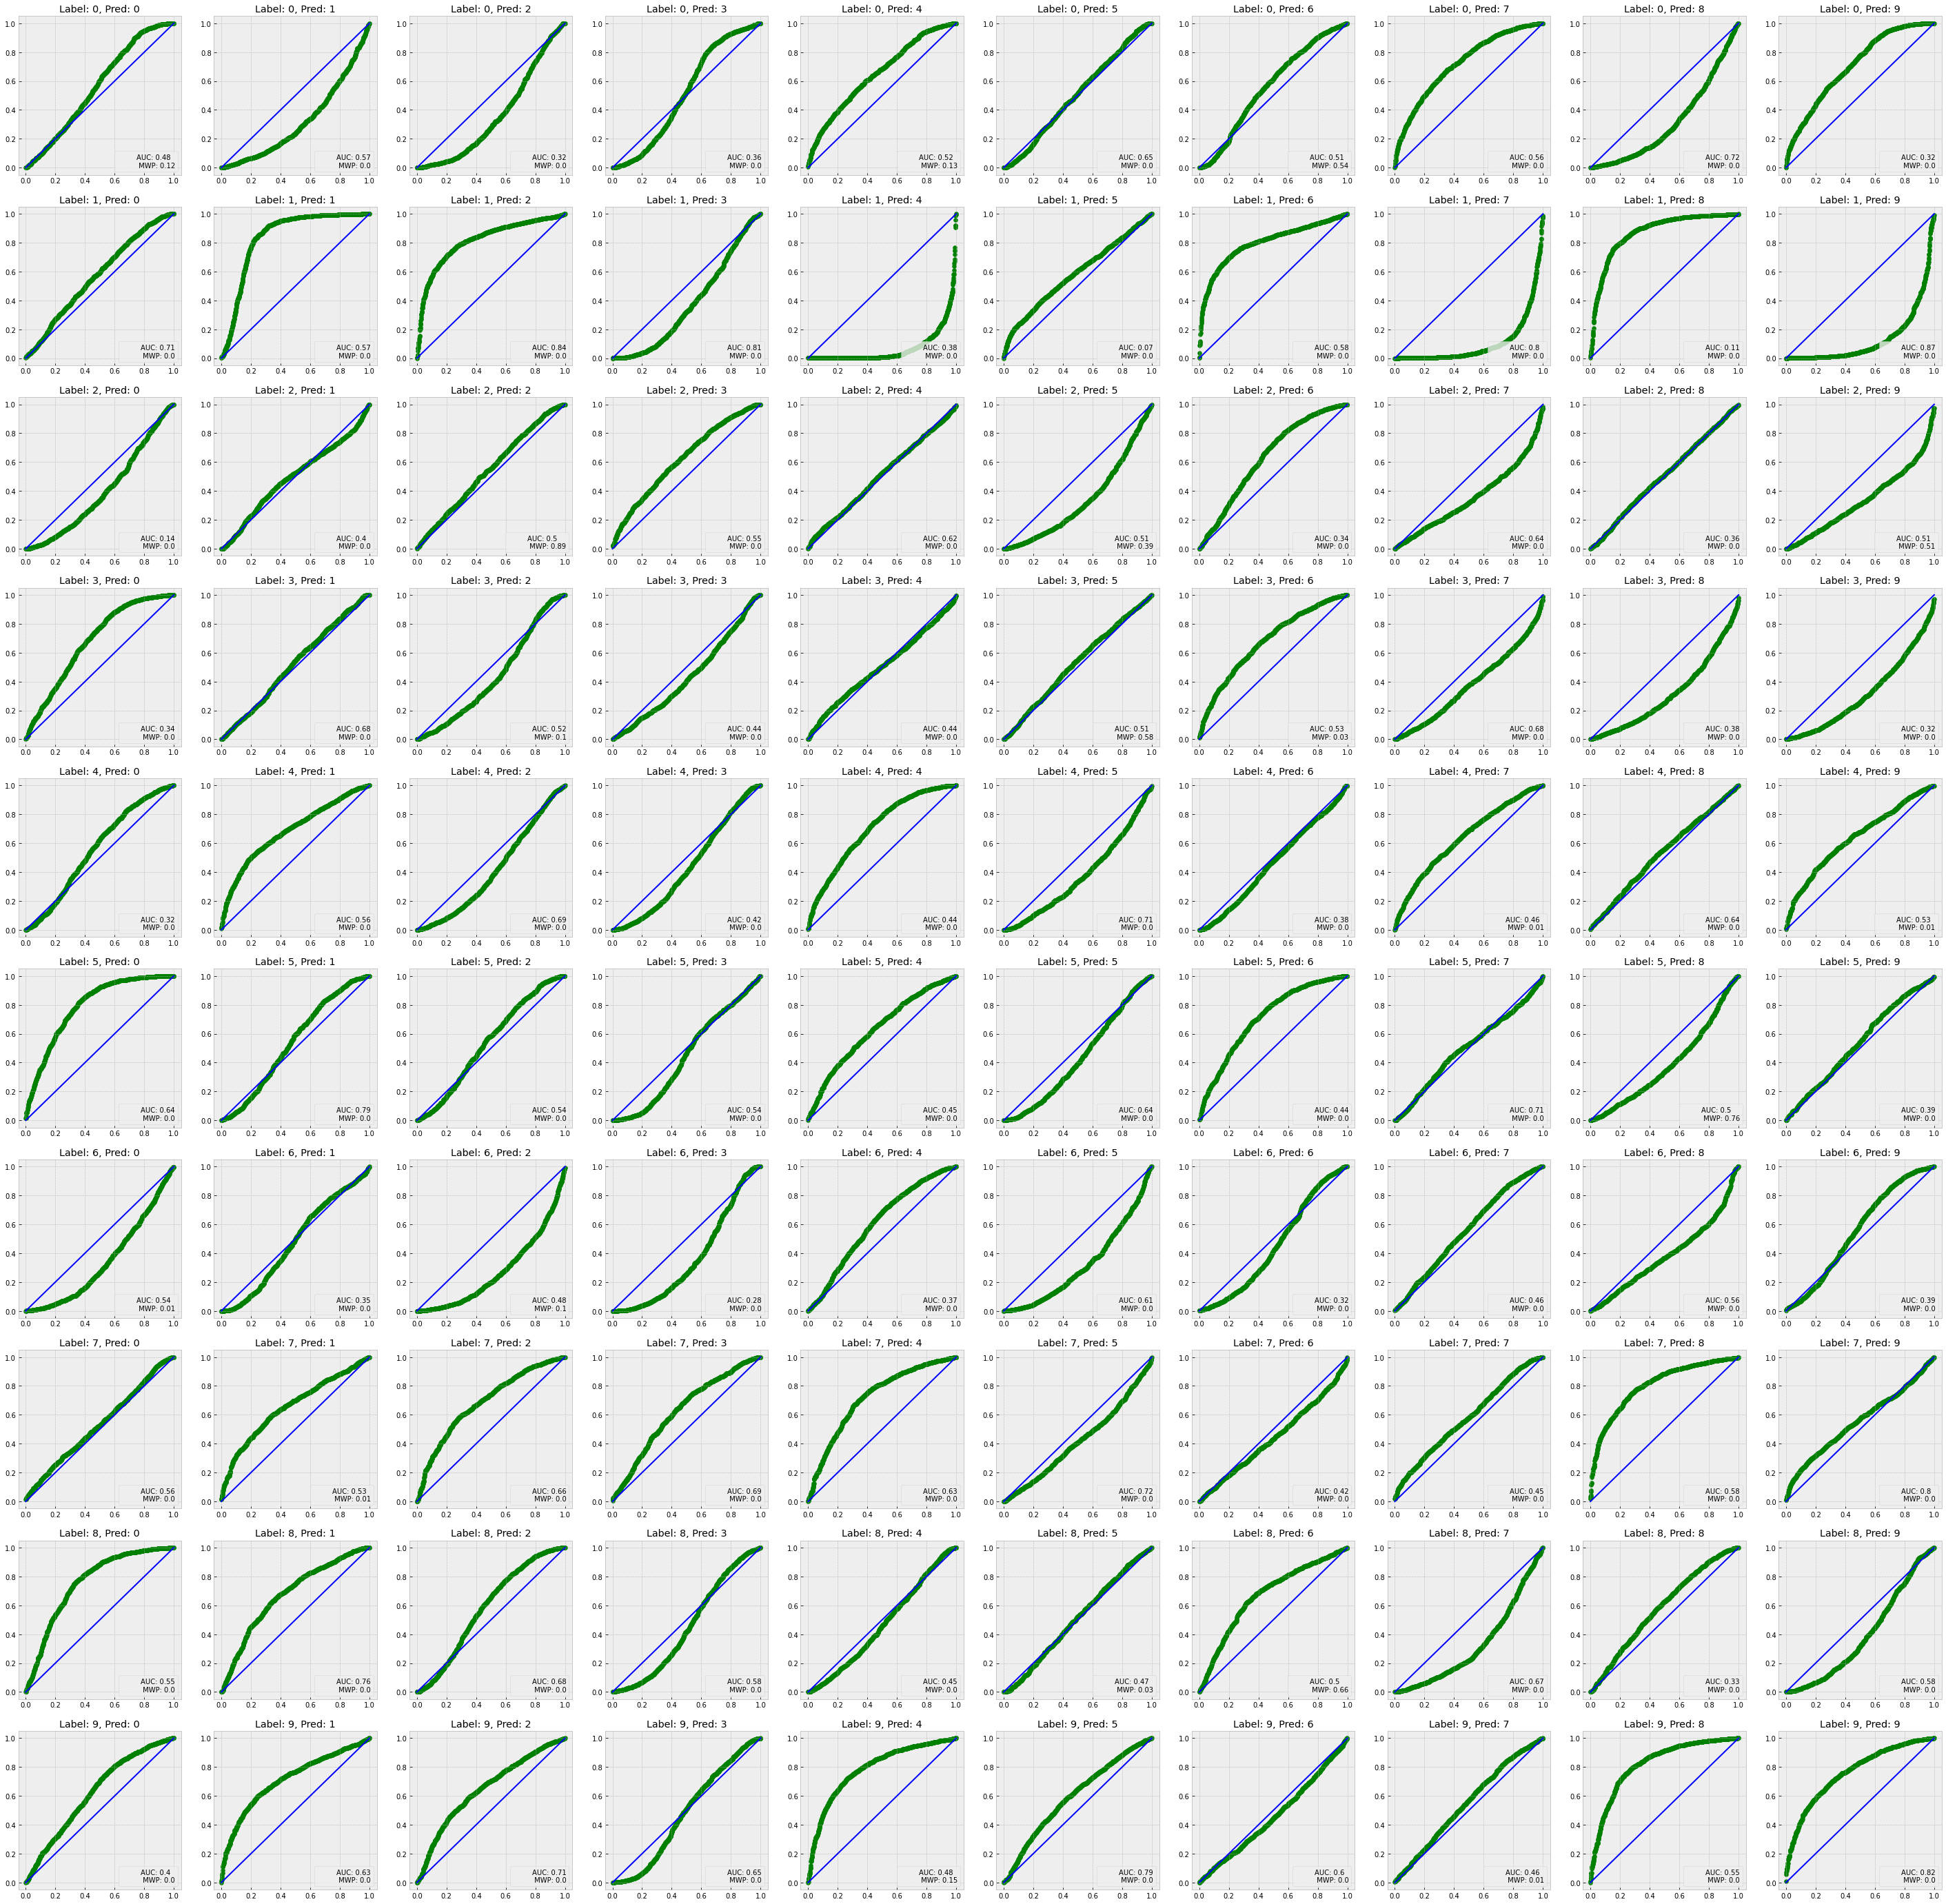
\includegraphics[width=2in]{img/bad_QQQ.png} & 
		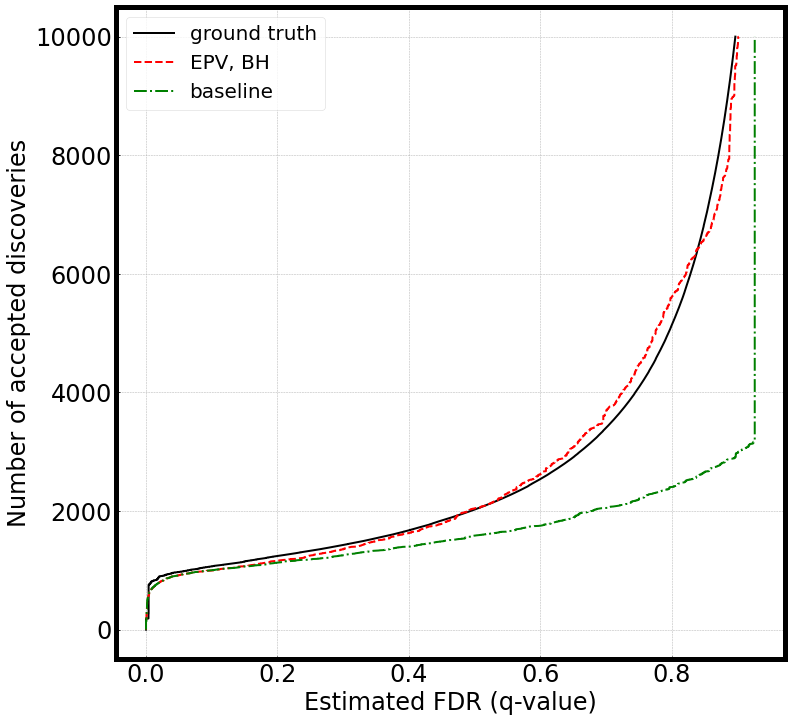
\includegraphics[width=2in]{img/cnn_shift_stats_prove.png}
		\\	
		A & B & C
	\end{tabular}
	\caption{{\bf  Influence of statistical correction.}
        (A) shows the QQ plots for each class of predictions, separated by true class labels in the classical case. (B) has an identical meaning to panel (A) except for using the shifted test data. (C) illustrates the number of trusted classifications as a function of the FDR when it is controlled with true labels (black line), with BHP, based on statistically adjusted EPV (red line) and static ones (green line) in the shifted case.}
	\label{fig:influence}
\end{figure}

For the sake of coherence, we find it mandatory to present particular reasons for introducing the aforementioned statistical correction. Actually, the first version of EPV did not involve this step. However, both balanced and shift cases have shown a significant drawback of such an approach. Figure \ref{fig:influence} represents such a situation. \ref{fig:influence}A shows the QQ plots from the multiclass case, each representing the p-values distribution, with the true label being placed on y-axis and the predicted one - on the x-axis (hence, the p-values for correct predictions are located on the diagonal). We can see positive results for EPV in terms of the perfect diagonal. However, when the data distribution shift takes place (\ref{fig:influence}B), a serious degradation can be identified. If moving further to the FDR control graph, we see a huge difference between poor performance of the static EPV (green line) and the statistically adjusted ones (red line).

The explanation lies in the nature of the  model's scores distribution. It was empirically found that when bringing the shift procedure to the experiment, our CNN starts extending the possible range of scores since facing the unexpected data representation. Hence, the static EPV procedure is challenged by lots of negative values being moved leftwards, which is the reason of such a slashing jump at the end of the curve - too many test samples have a unit p-value, appearing below the left border of the null hypothesis.

At the same time, if perceiving our data in terms of two distributions - positive and negative - then we can infer the corresponding statistical features. The mean and standard deviation are the one giving profound description. Hence, we found it rational to adjust the test distributions, separated by a border equal to local minima of kde function, so that they inherit training $\mu$ and $\sigma$ parameters. The results have empirically proven our thesis.

\subsection{Searching for accuracy advancement}

We also made an attempt to ameliorate the accuracy of the classification itself via EPV. Predicting solely on such p-values seemed to bring no effect. Among many methods, several were the most promising: the k-nearest neighbours algorithm and the angular softmax. However, they all faced significant challenges and did not ameliorate our performance.

\section{Conclusion}

To sum up, we should outline that the foundation of the work has been laid with a pure understanding of an established goal. We have successfully controlled the FDR level in each of the cases because of the profound implementation of the entire procedure, taking into account all possible ramifications. While we did not achieve our secondary objective of enhancing the model’s classification performance, we still get results very close to the ground truth, surpassing the rival LTT algorithm. The EPV are uniformly distributed, which allows to plot highly efficient curves on the “FDR control” graphs. Hence, we hope to continue our research, bringing the method to more real-life challenges. Such a validation would take our approach to a new level and perhaps make it a common solution for dozens of classification tasks.

	
%
%Exact methods ... 
%Let us discuss this method in detail. This method requires the following elements:
%\begin{enumerate}
%	\itemsep-3pt  		
%	\item Mass ...
%	
%	\item Exact methods employ ...
%\end{enumerate}
%
%The XPV method begins by placing a 1.0 to the $D[n,0]$, where $n$ indicates the discretized mass of the N-terminal group. This means that, there is exactly one N-terminal residue but its corresponding score is exactly 0, because N-terminal residues are not considered in the scoring. The elements of the dynamic programming table are filled recursively. Let us consider the cell $D[r,c]=n$, where there are exactly $n$ peptide fragments whose discretized mass is $c$ and they all score exactly $r$. Consequently, when all of these $n$ different peptide fragments are appended with an amino acid $X$, then there are $n$ peptides with a discretized mass of 
%\begin{equation}
%b=c+d_w(X)
%\label{eq:new_column}
%\end{equation}
% and their score
%
%\section{Data sets and methods}
%
%
%\subsection{Data sets}
%In our experiments, we used four, publicly availabl
%
%\begin{table}[t]
%	\centering
%	\caption{Summary of mass spectrometry data sets}
%	\label{tb:dataset_ms_summary}
%	\begin{tabular*}{\textwidth}{l@{\extracolsep{\fill}}llrr} 
%		\hline
%		ID& Name&Instrument& Num. of spectra & ACP$^1$\\
%		\hline
%		HumVar & H. Sapiens, Human Variation& LTQ Orbitrap& 15,057 & 2771.89  \\
%		Malaria& P. Falciparum & LTQ Orbitrap& 12,594  & 1024.06\\	
%		Kingdom& H. Sapiens  & Q Exactive HF-X Orbitrap	&  178,024& 2124.93\\
%		LUAD &  H. Sapiens, Lung Adeno Carcinoma & Q Exactive HF-X Orbitrap & 41,613 &2771.92\\
%		\hline		
%	\end{tabular*}\\
%	\raggedright \footnotesize Notes: The precursor ion tolerance was set to 10 ppm for all data sets, no isotope error was allowed. $^1$Average candidate peptide per spectrum.
%\end{table}
%
%\section{Results and discussion}
%\subsection{Main results}
%We begin 
%\begin{figure}[h]
%   \centering
%   \footnotesize
%   \setlength{\tabcolsep}{0pt}	
%  % \begin{tabular}{cc}	
%%		(A)\raisebox{-0.90\height}{\includegraphics[trim=0cm 0cm 0cm 0cm,clip=true, width=0.45\textwidth]{HUMVAR.pdf}} &
%%		(B)\raisebox{-0.90\height}{\includegraphics[trim=0cm 0cm 0cm 0cm,clip=true, width=0.45\textwidth]{MALARIA.pdf}}\\ 
%%		(C)\raisebox{-0.90\height}{\includegraphics[trim=0cm 0cm 0cm 0cm,clip=true, width=0.45\textwidth]{KINGDOM.pdf}}& 
%%		(D)\raisebox{-0.90\height}{\includegraphics[trim=0cm 0cm 0cm 0cm,clip=true, width=0.45\textwidth]{LUAD.pdf}} \\
%%	\end{tabular}
%\caption{The number of PSMs accepted at various FDR levels obtained with refactored XCorr, Tailor, and XPV methods using HRFS and LRFS in our benchmark data sets.}
%\label{fg:hrxpv-perf}
%\end{figure}


\section*{Author contributions}
\ifdefined\DOUBLEBLINDREVIEW
Omitted for double-blind peer-review.
\else
AKF concieved the idea that accurate empirical p-values would be derived from training data. AB worked out the methods and carried out experiments. AKF and AB wrote the manuscript.
\fi

\section*{Competing financial interests}
The authors declare no competing financial interests.


\section*{Availability}
\todo{AB}{Prepare a github page with the jupyter notebook experiments.}

%
%\begin{suppinfo}
%	The following supporting information is available free of charge at ACS website \url{http://pubs.acs.org}.
%	\begin{itemize}		
%		\itemsep0cm 	
%		\item Supplementary Note S1: Detailed description of the experimental data used. 
%		\item Supplementary Note S2: Detailed description of the methods used.
%		\item Supplementary Algorithm S1: Detailed pseudo code of the standard exact p-value (XPV) algorithm for XCorr scoring.
%		\item Supplementary Algorithm S2: Detailed pseudo code of the high -resolution exact p-value (HR-XPV) algorithm for XCorr scoring of high resolution MS/MS data.
%		\item Supplementary Data File S1 ({\bf \url{scripts.zip} (Zipped Linux bash scripts)}.): Script files to reproduce our experiments containing all the parameters used.
%	\end{itemize}	
%\end{suppinfo}

%\printbibliography	
\bibliographystyle{plain}           % Style BST file.
\bibliography{bibliography}

\end{document}
